\documentclass[12pt,a4paper]{article}
\usepackage[utf8]{inputenc}%Para Tildes y ñ%
\usepackage[spanish]{babel}
\usepackage{amsmath}
\usepackage{amsfonts}
\usepackage{amssymb}
\usepackage{adjustbox}
\usepackage{graphicx} 
\usepackage{pdfpages} %para importar paginas de un pdf 
\usepackage{booktabs}
\usepackage[bookmarks = true, colorlinks=true, linkcolor = black, citecolor = green, menucolor = black, urlcolor = black]{hyperref} 
\usepackage[left=2cm,right=2cm,top=2cm,bottom=2cm]{geometry} 
\usepackage{multirow}
\usepackage{circuitikz}
\usepackage{siunitx}
\usepackage{tabularx}
\usepackage{listings}
\usepackage{verbatimbox}
\usepackage{multicol}
\usepackage{xcolor}
\usepackage{verbatimbox}
\usepackage{float}
\usepackage{textcomp}
\usepackage{caption}
\usepackage{subcaption}
\setcounter{secnumdepth}{0} % ///////////////////////////////////////////// Para que los \section no tenga numeros
\DeclareRobustCommand{\Colon}{{%
  \ooalign{%
    \hidewidth\raisebox{0.2ex}{/}\kern0.1em\hidewidth\cr
    C\cr
    \hidewidth\kern0.1em\raisebox{0.2ex}{/}\hidewidth\cr
  }%
}}
%Code listing style named "mystyle"
\lstdefinestyle{mystyle}{
  backgroundcolor=\color{backcolour}, commentstyle=\color{codegreen},
  keywordstyle=\color{magenta},
  numberstyle=\tiny\color{codegray},
  stringstyle=\color{codepurple},
  basicstyle=\ttfamily\footnotesize,
  breakatwhitespace=false,         
  breaklines=true,                 
  captionpos=b,                    
  keepspaces=true,                 
  numbers=left,                    
  numbersep=5pt,                  
  showspaces=false,                
  showstringspaces=false,
  showtabs=false,                  
  tabsize=2
}

\input{vspm.hd}

\newcommand{\keywords}[1]{\par\addvspace\baselineskip
\noindent\keywordname\enspace\ignorespaces#1}
\addto\captionsspanish{\renewcommand{\listtablename}{Índice de tablas}}		% Cambiar nombre a lista de tablas   
\addto\captionsspanish{\renewcommand{\tablename}{Tablas}}					% Cambiar nombre a tablas

\usepackage{pdfpages}
\usepackage{enumerate}%listas y viñetas
\author{ Leonardo Serrano Arias C17484  \\Lorena Solís Extteny B97657\\{\small }\\ \\ Profesor: Marco Villalta  \vspace*{3.0in}}
\title{Universidad de Costa Rica\\{\small Facultad de Ingeniería\\Escuela de Ingeniería Eléctrica\\IE0624 – Laboratorio de Microcontroladores\\II ciclo 2024\\\vspace*{0.55in} Laboratorio \# 5 }\\ STM32/Arduino: GPIO, Giroscopio, comunicaciones, TinyML \vspace*{1.35in}}
\date{20 de Noviembre, 2024} 

\lstset{style=mystyle}
\begin{document} 

\maketitle  
\thispagestyle{empty}%%no numerar la portada
\renewcommand{\thepage}{\roman{page}}
\newpage
\tableofcontents

\listoffigures 

%\listoftables  

%%%%%%%%%%  
\renewcommand{\thepage}{\arabic{page}} 
\setcounter{page}{1}

\newpage
\section{Introducción}
En este laboratorio se desarrolló un modelo para el reconocimiento de actividad humana utilizando un microcontrolador Arduino Nano 33 BLE Sense. Este modelo tiene como objetivo identificar tres movimientos principales: círculo, estacionario y "arriba-abajo", basándose en datos de aceleración, velocidad angular y orientación proporcionados por un sensor inercial (IMU LSM9DS1). A lo largo del proyecto, se implementaron diversas etapas, desde la captura de datos y su procesamiento, hasta la creación de un modelo de aprendizaje automático en la plataforma Edge Impulse, logrando su implementación en hardware embebido. Los resultados obtenidos demostraron un alto nivel de exactitud, superando el 99\% en las clasificaciones para los movimientos definidos, y una capacidad robusta para identificar anomalías. Finalmente, el modelo entrenado fue integrado al microcontrolador mediante una biblioteca compatible con Arduino IDE, garantizando su funcionamiento autónomo y eficiente.

El repositorio utilizado para el desarrollo de este laboratorio se encuentra en la siguiente dirección: \url{https://github.com/Leonardo-SA/IE-0624_II_2024_C17484_B97657.git}


\section{Nota Teórica}

\subsection{Arduino Nano 33 BLE}
El \textit{Arduino Nano 33 BLE} \cite{hoja} es una placa de desarrollo compacta, diseñada para aplicaciones de bajo consumo energético y comunicaciones inalámbricas mediante \textit{Bluetooth Low Energy} (BLE). Esta placa está basada en el microcontrolador nRF52840 de Nordic Semiconductor, un procesador ARM Cortex-M4 de 32 bits con punto flotante, que ofrece una combinación de capacidades de procesamiento, eficiencia energética y conectividad. A continuación se presentan sus características técnicas:

\begin{itemize}
    \item \textbf{Microcontrolador}: 
    
        \subitem \textbf{Modelo}: nRF52840 
        \subitem \textbf{Arquitectura}: Procesador ARM Cortex-M4F a 64 MHz, con soporte para punto flotante, facilitando el procesamiento de señales y la ejecución de algoritmos de aprendizaje automático ligero.
    
    \item \textbf{Voltaje de funcionamiento}: 3.3V.

    \item \textbf{Memoria}: 
    
        \subitem \textit{Flash}: 1 MB, para almacenamiento de programas y datos de sensores.
        \subitem \textit{SRAM}: 256 KB, optimizada para operaciones de cálculo en tiempo real y almacenamiento de variables temporales.
 

    \item \textbf{Pines de E/S}: 

        \subitem 14 pines digitales (PWM habilitado).
        \subitem 8 pines de entrada analógica. 
    \
    Permite la integración de múltiples dispositivos y sensores externos.

    \item \textbf{Sensores integrados}: 
  
        \subitem \textbf{IMU}: LSM9DS1 de 9 ejes (acelerómetro, giroscopio y magnetómetro).
        \subitem \textbf{Sensor de proximidad y luz}: APDS9960 (detección de proximidad, color RGB, intensidad de luz y gestos).
        \subitem \textbf{Audio y Video}: Micrófono digital MP34DT05 y cámara OV7675 (solo en la versión BLE Sense).


    \item \textbf{Comunicación}: Compatible con interfaces UART, SPI e I2C, facilitando la integración con dispositivos de comunicación y otros periféricos.

    \item \textbf{Dimensiones}: 45x18 mm, ideal para proyectos portátiles y aplicaciones IoT.
\end{itemize}

Adicionalmente, se agrega el diagrama de pines acontinuación:  
\begin{figure}[H]
    \centering
    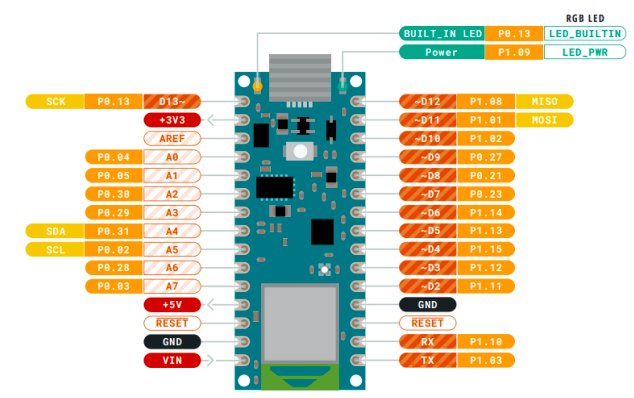
\includegraphics[width=0.6\linewidth]{Imagenes/pines.png}
    \caption{Diagrama de pines del Arduino Nano BLE 33 \cite{hoja}}
    \label{fig:1}
\end{figure}
Seguidamente, se muestra la topología de la placa:
\begin{figure}[H]
    \centering
    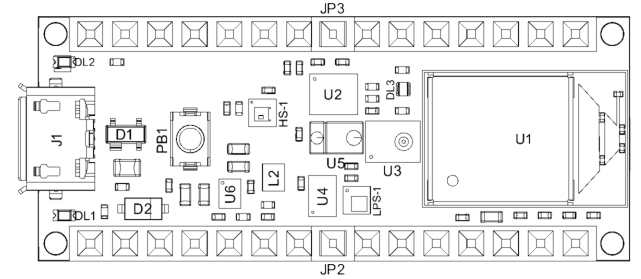
\includegraphics[width=0.6\linewidth]{Imagenes/topologia.png}
    \caption{Topología del Arduino Nano BLE 33 \cite{hoja}}
    \label{fig:2}
\end{figure}

A continuación, se muestra el árbol de potencia del microcontrolador:
\begin{figure}[H]
    \centering
    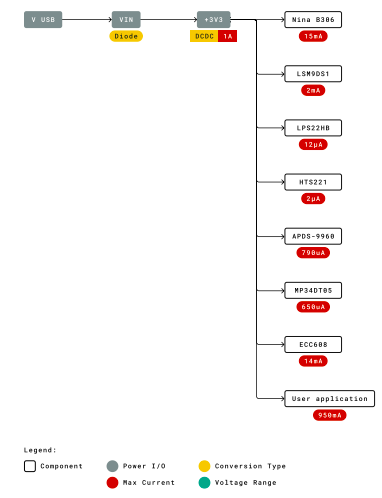
\includegraphics[width=0.3\linewidth]{Imagenes/V_tree.png}
    \caption{Arbol de potencia del Arduino Nano BLE 33 \cite{hoja}}
    \label{fig:3}
\end{figure}

Por otro lado, en la siguiente imagen se puede observar el diagrama de bloques del microcontrolador nRF52840:


\begin{figure}[H]
    \centering
    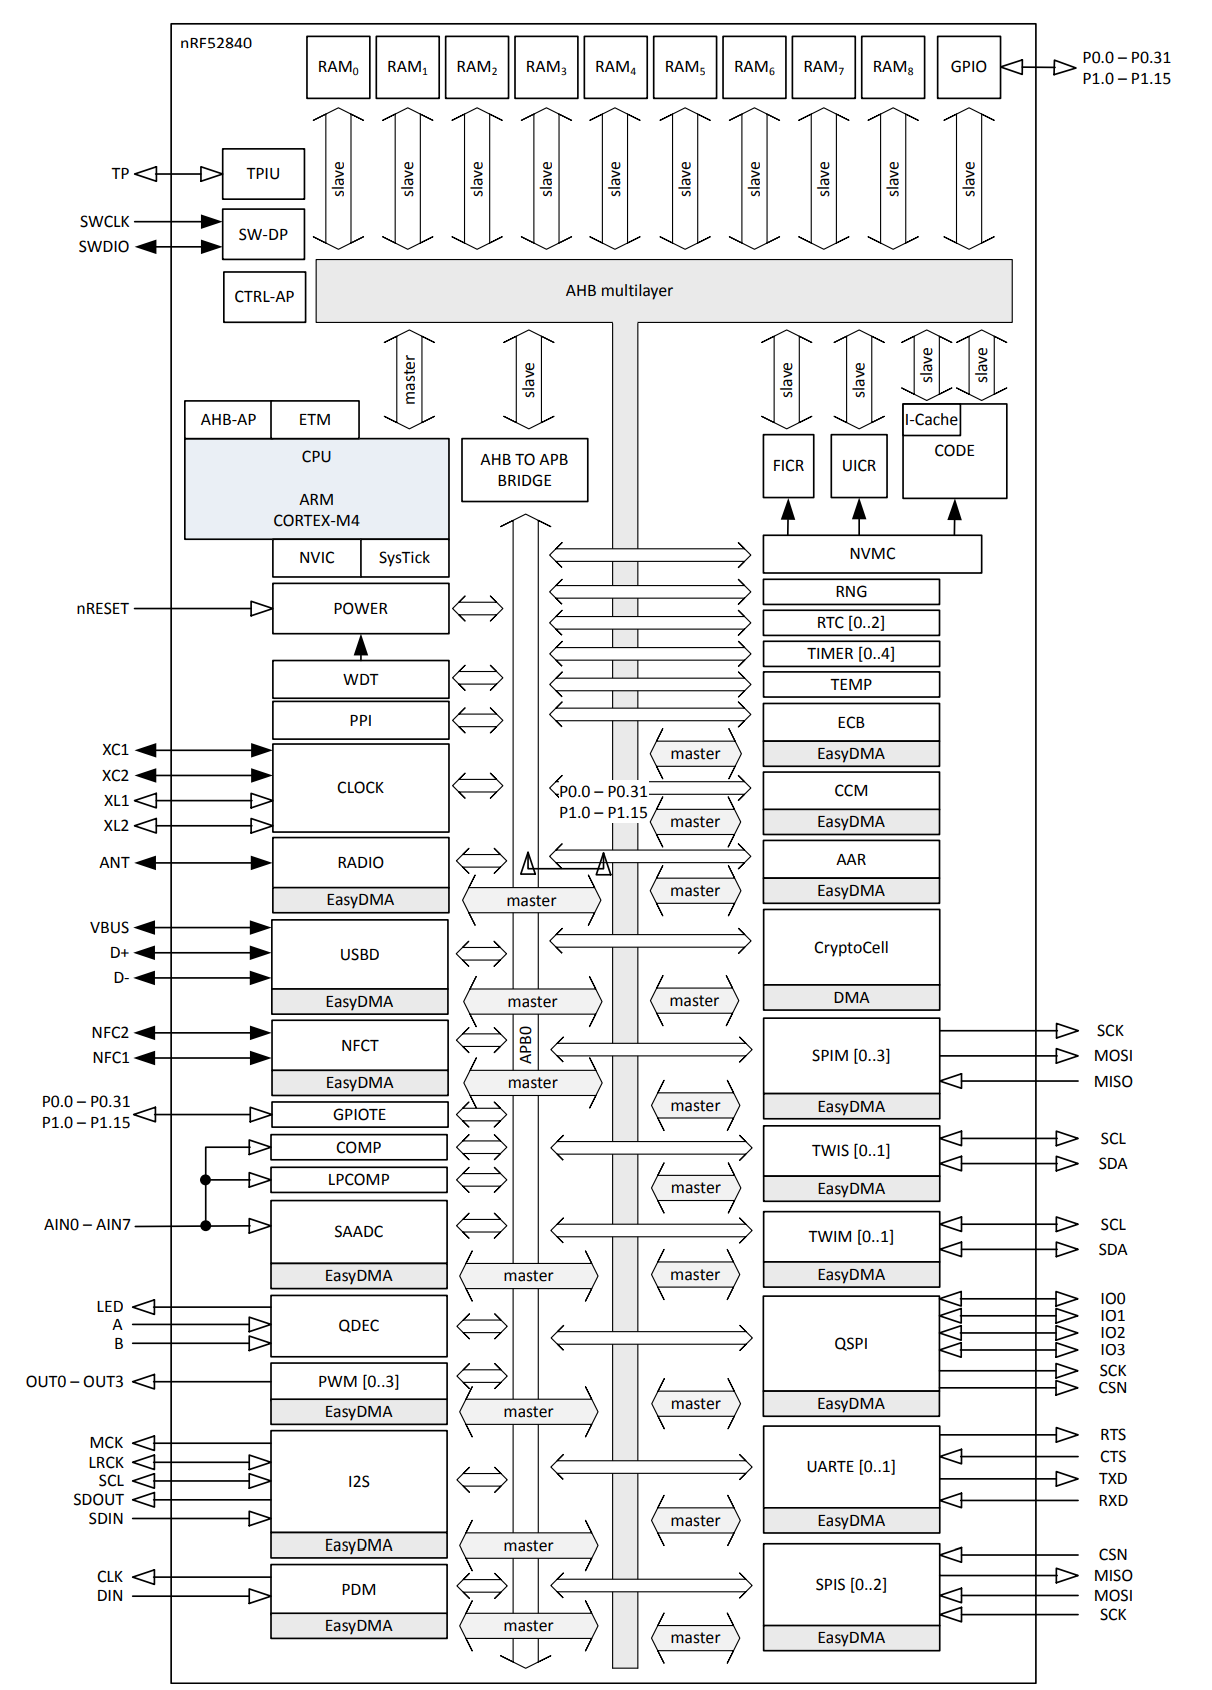
\includegraphics[width=0.61\linewidth]{Imagenes/bloques.png}
    \caption{Diagrama de bloques del MCU nRF52840 \cite{nRF52840}}
    \label{fig:3}
\end{figure}


\subsection{Componentes del Arduino Nano 33 BLE}

\subsubsection{IMU LSM9DS1}
El LSM9DS1 \cite{imu} es un sistema en paquete que combina sensores de aceleración, velocidad angular y magnetómetro. Este dispositivo es clave en aplicaciones de reconocimiento de actividad humana (HAR) ya que permite detectar la orientación, rotación y movimiento de la placa.

\begin{itemize}
    \item \textbf{Acelerómetro}: 
 
        \subitem Rango de medida: configuraciones ajustables de ±2g, ±4g, ±8g o ±16g, permitiendo capturar aceleraciones desde movimientos suaves hasta rápidos.
        \subitem Resolución: mide aceleraciones lineales en 3 ejes con una resolución que depende del rango configurado.
        \subitem Aplicaciones: útil para detectar cambios de posición, inclinación y patrones de movimiento en aplicaciones de HAR.
    
    
    \item \textbf{Giroscopio}: 
  
        \subitem Rango de medida: configuraciones de ±245, ±500 y ±2000 dps (grados por segundo), adaptándose a diferentes tipos de rotación y velocidad.
        \subitem Resolución: mide velocidades angulares en 3 ejes, permitiendo detectar rotaciones en tiempo real.
        \subitem Aplicaciones: esencial para captar rotaciones rápidas, como giros, y movimientos de rotación, útiles en sistemas de reconocimiento de gestos y actividad física.
   
    
    \item \textbf{Magnetómetro}: 
    
        \subitem Rango de medida: configuraciones de ±4, ±8, ±12 y ±16 gauss, ajustables para diferentes niveles de sensibilidad.
        \subitem Aplicaciones: permite la orientación mediante la detección del campo magnético terrestre, complementando las lecturas del acelerómetro y giroscopio para obtener datos completos de la orientación de la placa.
   
\end{itemize}

El LSM9DS1 utiliza interfaces I2C y SPI para comunicación, y permite configurar los sensores en modos de bajo consumo para reducir la demanda energética, ideal para aplicaciones portátiles y de IoT.

\subsubsection{Sensor de proximidad, color, y gestos APDS9960}
El sensor APDS9960 \cite{sensor} es un dispositivo multifuncional que integra la detección de proximidad, medición de luz ambiente, y reconocimiento de gestos. Estas capacidades son útiles en proyectos de interacción y en aplicaciones de HAR donde es necesario detectar movimientos específicos de la mano u objetos cercanos. Sus características incluyen:

\begin{itemize}
    \item \textbf{Detección de gestos}: Utiliza cuatro fotodiodos direccionales para medir la energía infrarroja (IR) reflejada y así detectar movimientos en direcciones específicas (arriba, abajo, izquierda, derecha).
    \item \textbf{Sensor de luz ambiental y color}: Capta niveles de luz RGB y detecta la intensidad de la luz ambiental, ajustándose automáticamente a la iluminación del entorno.
    \item \textbf{Sensor de proximidad}: Detecta objetos cercanos midiendo la intensidad de la luz IR reflejada. Puede configurarse para activar funciones cuando se detecta un objeto a cierta distancia.
\end{itemize}

\begin{figure}[H]
    \centering
    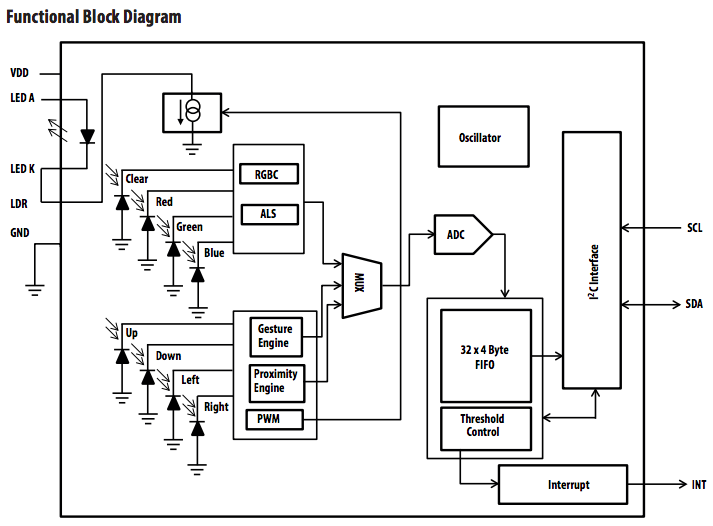
\includegraphics[width=0.6\linewidth]{Imagenes/A_BD.png}
    \caption{Diagrama de bloques del sensor de proximidad APDS9960 \cite{sensor}}
    \label{fig:4}
\end{figure}

\subsubsection{Micrófono digital MP34DT05 y cámara OV7675}
El micrófono MP34DT05 \cite{micro} y la cámara OV7675 \cite{cam} añaden funcionalidades de captura de audio e imagen al Arduino Nano 33 BLE, abriendo posibilidades para aplicaciones de monitoreo en tiempo real y control mediante voz o imagen.

\begin{itemize}
    \item \textbf{Micrófono MP34DT05}:

        \subitem Resolución: Capta sonidos del ambiente y permite realizar análisis de audio o comandos de voz.
        \subitem Aplicaciones: Usado en aplicaciones de reconocimiento de voz, monitoreo de audio o sistemas de activación por sonido.
  
    \item \textbf{Cámara OV7675}:
   
        \subitem Resolución máxima: 640x480 píxeles (VGA), proporcionando imágenes claras para capturas básicas.
        \subitem Aplicaciones: Ideal para proyectos de reconocimiento de gestos visuales, detección de movimiento, o cualquier aplicación que requiera entrada visual.

\end{itemize}

\begin{figure}[H]
    \centering
    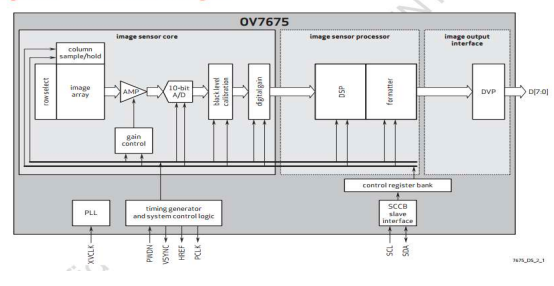
\includegraphics[width=0.9\linewidth]{Imagenes/OV_BD.png}
    \caption{Diagrama de bloques del módulo de la cámara OV7675 \cite{cam}}
    \label{fig:5}
\end{figure}

\subsection{Registros y periféricos}
Los registros que utiliza este microcontrolador se muestran en la siguiente tabla \cite{nRF52840}:

\begin{table}[h!]
\centering
\caption{Instancias}
\adjustbox{max width=\textwidth}{
\begin{tabularx}{\textwidth}{|c|c|c|X|X|}
\hline
\textbf{Dirección Base} & \textbf{Periférico} & \textbf{Instancia} & \textbf{Descripción} & \textbf{Configuración} \\ \hline
0x50000000 & GPIO & GPIO & Entrada y salida de propósito general & Obsoleto \\ \hline
0x50000000 & GPIO & P0 & Entrada y salida de propósito general, puerto 0 & Implementado P0.00 a P0.31 \\ \hline
0x50000300 & GPIO & P1 & Entrada y salida de propósito general, puerto 1 & Implementado P1.00 a P1.15 \\ \hline
\end{tabularx}
}
\label{tab:instancias}
\end{table}

\begin{table}[h!]
\centering
\caption{Registros}
\adjustbox{max width=\textwidth}{
\begin{tabularx}{\textwidth}{|c|c|X|}
\hline
\textbf{Registro} & \textbf{Desplazamiento} & \textbf{Descripción} \\ \hline
OUT & 0x504 & Escribe en el puerto GPIO \\ \hline
OUTSET & 0x508 & Establece bits individuales en el puerto GPIO \\ \hline
OUTCLR & 0x50C & Borra bits individuales en el puerto GPIO \\ \hline
IN & 0x510 & Lee el puerto GPIO \\ \hline
DIR & 0x514 & Dirección de los pines GPIO \\ \hline
DIRSET & 0x518 & Registro de configuración DIR \\ \hline
DIRCLR & 0x51C & Registro para borrar configuración DIR \\ \hline
LATCH & 0x520 & Registro de retención que indica qué pines GPIO cumplen criterios \\ \hline
DETECTMODE & 0x524 & Selecciona entre comportamiento por defecto y modo LDETECT \\ \hline
PIN\_CNF[0] & 0x700 & Configuración de los pines GPIO \\ \hline


\end{tabularx}
}
\label{tab:registros}
\end{table}

\begin{table}[h!]
\centering
\caption{Continuación de registros}
\adjustbox{max width=\textwidth}{
\begin{tabularx}{\textwidth}{|c|c|X|}
\hline
\textbf{Registro} & \textbf{Desplazamiento} & \textbf{Descripción} \\ \hline
PIN\_CNF[1] & 0x704 & Configuración de los pines GPIO \\ \hline
PIN\_CNF[2] & 0x708 & Configuración de los pines GPIO \\ \hline
PIN\_CNF[3] & 0x70C & Configuración de los pines GPIO \\ \hline
PIN\_CNF[4] & 0x710 & Configuración de los pines GPIO \\ \hline
PIN\_CNF[5] & 0x714 & Configuración de los pines GPIO \\ \hline
PIN\_CNF[6] & 0x718 & Configuración de los pines GPIO \\ \hline
PIN\_CNF[7] & 0x71C & Configuración de los pines GPIO \\ \hline
PIN\_CNF[8] & 0x720 & Configuración de los pines GPIO \\ \hline
PIN\_CNF[9] & 0x724 & Configuración de los pines GPIO \\ \hline
PIN\_CNF[10] & 0x728 & Configuración de los pines GPIO \\ \hline
PIN\_CNF[11] & 0x72C & Configuración de los pines GPIO \\ \hline
PIN\_CNF[12] & 0x730 & Configuración de los pines GPIO \\ \hline
PIN\_CNF[13] & 0x734 & Configuración de los pines GPIO \\ \hline
PIN\_CNF[14] & 0x738 & Configuración de los pines GPIO \\ \hline
PIN\_CNF[15] & 0x73C & Configuración de los pines GPIO \\ \hline
PIN\_CNF[16] & 0x740 & Configuración de los pines GPIO \\ \hline
PIN\_CNF[17] & 0x744 & Configuración de los pines GPIO \\ \hline
PIN\_CNF[18] & 0x748 & Configuración de los pines GPIO \\ \hline
PIN\_CNF[19] & 0x74C & Configuración de los pines GPIO \\ \hline
PIN\_CNF[20] & 0x750 & Configuración de los pines GPIO \\ \hline
PIN\_CNF[21] & 0x754 & Configuración de los pines GPIO \\ \hline
PIN\_CNF[22] & 0x758 & Configuración de los pines GPIO \\ \hline
PIN\_CNF[23] & 0x75C & Configuración de los pines GPIO \\ \hline
PIN\_CNF[24] & 0x760 & Configuración de los pines GPIO \\ \hline
PIN\_CNF[25] & 0x764 & Configuración de los pines GPIO \\ \hline
PIN\_CNF[26] & 0x768 & Configuración de los pines GPIO \\ \hline
PIN\_CNF[27] & 0x76C & Configuración de los pines GPIO \\ \hline
PIN\_CNF[28] & 0x770 & Configuración de los pines GPIO \\ \hline
PIN\_CNF[29] & 0x774 & Configuración de los pines GPIO \\ \hline
PIN\_CNF[30] & 0x778 & Configuración de los pines GPIO \\ \hline
PIN\_CNF[31] & 0x77C & Configuración de los pines GPIO \\ \hline
\end{tabularx}
}
\label{tab:registros}
\end{table}

Por otra parte, la instanciación de los periféricos se muestra a continuación:

\begin{table}[h!]
\centering
\caption{Instanciación de los periféricos}
\adjustbox{max width=\textwidth}{
\begin{tabularx}{\textwidth}{|c|c|c|c|X|}
\hline
\textbf{ID} & \textbf{Dirección Base} & \textbf{Periférico} & \textbf{Instancia} & \textbf{Descripción} \\ \hline
0 & 0x40000000 & CLOCK & CLOCK & Control de reloj \\ \hline
0 & 0x40000000 & POWER & POWER & Control de energía \\ \hline
0 & 0x50000000 & GPIO & GPIO & Entrada y salida de propósito general (obsoleto) \\ \hline
0 & 0x50000000 & GPIO & P0 & Entrada y salida de propósito general, puerto 0 \\ \hline
0 & 0x50000300 & GPIO & P1 & Entrada y salida de propósito general, puerto 1 \\ \hline
0 & 0x40001000 & RADIO & RADIO & Radio de 2.4 GHz \\ \hline
\end{tabularx}
}
\label{tab:perifericos}
\end{table}

\begin{table}[h!]
\centering
\caption{Contiuación de la instanciación de los periféricos}
\adjustbox{max width=\textwidth}{
\begin{tabularx}{\textwidth}{|c|c|c|c|X|}
\hline
\textbf{ID} & \textbf{Dirección Base} & \textbf{Periférico} & \textbf{Instancia} & \textbf{Descripción} \\ \hline
2 & 0x40002000 & UART & UART0 & Transmisor/receptor asincrónico universal (obsoleto) \\ \hline
2 & 0x40002000 & UARTE & UARTE0 & Transmisor/receptor asincrónico universal con EasyDMA, unidad 0 \\ \hline
3 & 0x40003000 & SPI & SPI0 & Maestro SPI 0 (obsoleto) \\ \hline
3 & 0x40003000 & SPIM & SPIM0 & Maestro SPI 0 \\ \hline
3 & 0x40003000 & SPIS & SPIS0 & Esclavo SPI 0 \\ \hline
3 & 0x40003000 & TWI & TWI0 & Interfaz de dos hilos, maestro 0 (obsoleto) \\ \hline
3 & 0x40003000 & TWIM & TWIM0 & Interfaz de dos hilos, maestro 0 \\ \hline
3 & 0x40003000 & TWIS & TWIS0 & Interfaz de dos hilos, esclavo 0 \\ \hline
4 & 0x40004000 & SPI & SPI1 & Maestro SPI 1 \\ \hline
4 & 0x40004000 & SPIM & SPIM1 & Maestro SPI 1 \\ \hline
4 & 0x40004000 & SPIS & SPIS1 & Esclavo SPI 1 \\ \hline
4 & 0x40004000 & TWI & TWI1 & Interfaz de dos hilos, maestro 1 (obsoleto) \\ \hline
4 & 0x40004000 & TWIM & TWIM1 & Interfaz de dos hilos, maestro 1 \\ \hline
4 & 0x40004000 & TWIS & TWIS1 & Interfaz de dos hilos, esclavo 1 \\ \hline
5 & 0x40005000 & NFCT & NFCT & Etiqueta de comunicación de campo cercano \\ \hline
6 & 0x40006000 & GPIOTE & GPIOTE & Tareas y eventos GPIO \\ \hline
7 & 0x40007000 & SAADC & SAADC & Convertidor de analógico a digital \\ \hline
8 & 0x40008000 & TIMER & TIMER0 & Temporizador 0 \\ \hline
9 & 0x40009000 & TIMER & TIMER1 & Temporizador 1 \\ \hline
10 & 0x4000A000 & TIMER & TIMER2 & Temporizador 2 \\ \hline
11 & 0x4000B000 & RTC & RTC0 & Contador de tiempo real 0 \\ \hline
12 & 0x4000C000 & TEMP & TEMP & Sensor de temperatura \\ \hline
13 & 0x4000D000 & RNG & RNG & Generador de números aleatorios \\ \hline
14 & 0x4000E000 & ECB & ECB & Cifrado electrónico de bloques (AES) \\ \hline
15 & 0x4000F000 & CCM & CCM & Contador AES con CBC-MAC \\ \hline
16 & 0x40010000 & WDT & WDT & Temporizador watchdog \\ \hline
17 & 0x40011000 & RTC & RTC1 & Contador de tiempo real 1 \\ \hline
18 & 0x40012000 & QDEC & QDEC & Decodificador de cuadratura \\ \hline
19 & 0x40013000 & COMP & COMP & Comparador de propósito general \\ \hline
20 & 0x40014000 & LPCOMP & LPCOMP & Comparador de baja potencia \\ \hline
21 & 0x40015000 & EGU & EGU0 & Unidad generadora de eventos 0 \\ \hline
22 & 0x40016000 & SWI & SWI0 & Interrupción por software 0 \\ \hline
23 & 0x40017000 & EGU & EGU1 & Unidad generadora de eventos 1 \\ \hline
24 & 0x40018000 & EGU & EGU2 & Unidad generadora de eventos 2 \\ \hline
25 & 0x40019000 & SWI & SWI5 & Interrupción por software 5 \\ \hline
26 & 0x4001A000 & TIMER & TIMER3 & Temporizador 3 \\ \hline
27 & 0x4001B000 & TIMER & TIMER4 & Temporizador 4 \\ \hline
28 & 0x4001C000 & PWM & PWM0 & Unidad de modulación por ancho de pulso 0 \\ \hline
30 & 0x4001E000 & ACL & ACL & Listas de control de acceso \\ \hline
\end{tabularx}
}
\label{tab:perifericos}
\end{table}


\begin{table}[h!]
\centering
\caption{Contiuación 2 de la instanciación de los periféricos}
\adjustbox{max width=\textwidth}{
\begin{tabularx}{\textwidth}{|c|c|c|c|X|}
\hline
\textbf{ID} & \textbf{Dirección Base} & \textbf{Periférico} & \textbf{Instancia} & \textbf{Descripción} \\ \hline
29 & 0x4001D000 & PDM & PDM & Interfaz de modulación por densidad de pulso (micrófono digital) \\ \hline
30 & 0x4001E000 & NVMC & NVMC & Controlador de memoria no volátil \\ \hline
31 & 0x4001F000 & PPI & PPI & Interconexión de periféricos programable \\ \hline
32 & 0x40020000 & MWU & MWU & Unidad de vigilancia de memoria \\ \hline
33 & 0x40021000 & PWM & PWM1 & Unidad de modulación por ancho de pulso 1 \\ \hline
34 & 0x40022000 & PWM & PWM2 & Unidad de modulación por ancho de pulso 2 \\ \hline
35 & 0x40023000 & SPI & SPI2 & Maestro SPI 2 (obsoleto) \\ \hline
35 & 0x40023000 & SPIM & SPIM2 & Maestro SPI 2 \\ \hline
35 & 0x40023000 & SPIS & SPIS2 & Esclavo SPI 2 \\ \hline
36 & 0x40024000 & RTC & RTC2 & Contador de tiempo real 2 \\ \hline
37 & 0x40025000 & I2S & I2S & Interfaz de sonido inter-IC \\ \hline
38 & 0x40026000 & FPU & FPU & Interrupción de unidad de punto flotante \\ \hline
39 & 0x40027000 & USBD & USBD & Dispositivo de bus serie universal \\ \hline
40 & 0x40028000 & UARTE & UARTE1 & Transmisor/receptor asincrónico universal con EasyDMA, unidad 1 \\ \hline
41 & 0x40029000 & QSPI & QSPI & Interfaz de memoria externa \\ \hline
42 & 0x5002A000 & CC\_HOST\_RGF & CC\_HOST\_RGF & Interfaz de plataforma host \\ \hline
43 & 0x5002A000 & CRYPTOCELL & CRYPTOCELL & Interfaz de control del subsistema CryptoCell \\ \hline
44 & 0x4002E000 & PWM & PWM3 & Unidad de modulación por ancho de pulso 3 \\ \hline
45 & 0x4002F000 & SPIM & SPIM3 & Maestro SPI 3 \\ \hline

\end{tabularx}
}
\label{tab:perifericos}
\end{table}






\subsection{Conceptos importantes}

\subsubsection{Machine Learning}
El aprendizaje automático (ML, por sus siglas en inglés) es una rama de la inteligencia artificial que se enfoca en el uso de datos y algoritmos para permitir que las máquinas simulen la forma en que los humanos adquieren conocimiento. Este proceso implica una mejora constante en la precisión de los resultados a medida que el modelo aprende de los datos proporcionados. ML tiene aplicaciones que van desde clasificaciones hasta predicciones, adaptándose a diversas áreas de la informática e industrias. \cite{ml}

El funcionamiento de los algoritmos de aprendizaje automático se divide en tres fases principales. En primer lugar, el proceso de decisión, donde el algoritmo analiza los datos de entrada para identificar patrones y realizar predicciones. Luego, se utiliza una función de error para medir la discrepancia entre las predicciones y los resultados esperados, evaluando así la precisión del modelo. Finalmente, un proceso de optimización ajusta los parámetros del modelo para mejorar su desempeño, iterando hasta alcanzar un nivel aceptable de precisión. Este ciclo de evaluación y mejora es esencial para el aprendizaje continuo del sistema. \cite{ml}

\subsubsection{Edge Impulse}
Edge Impulse es una plataforma para desarrollar algoritmos de aprendizaje máquina enfocados a implementarse en sistemas embebidos como microcontroladores o computadoras con recursos reducidos. Tiene disponibles diversas herramientas que la hacen adecuada tanto para principiantes como usuarios avanzados. La practicidad de esta herramienta es que no necesitas involucrarte demasiado con el código, puedes implementar tu algoritmo con ingresar tu base de datos, ajustas los hiperparámetros y entrenas el programa. \cite{ei}


\subsubsection{Tensorflow}
TensorFlow es una herramienta fundamental en el desarrollo de inteligencia artificial y aprendizaje automático. Es una biblioteca de código abierto diseñada para Machine Learning (ML), desarrollada por Google para abordar las necesidades que surgen al trabajar con redes neuronales artificiales. Esta plataforma permite construir y entrenar redes neuronales capaces de detectar patrones y replicar razonamientos propios del ser humano. Una de las principales ventajas de TensorFlow es su versatilidad. Además de su enfoque en redes neuronales, es una solución multiplataforma que puede ejecutarse en CPUs, GPUs e incluso en unidades de procesamiento especializadas como las TPUs (Tensor Processing Units), optimizando su rendimiento en distintos entornos. \cite{tensorflow}



\subsection{Librerías de Arduino IDE}
A continuación se detallan las librerías utilizadas en el Arduino \cite{lib}:


\subsubsection{\texttt{Laboratorio\_5\_inferencing.h}}
Esta librería forma parte del SDK de Edge Impulse y se emplea para ejecutar inferencias de modelos de machine learning en dispositivos embebidos. Facilita la integración de modelos preentrenados generados por Edge Impulse, permitiendo la clasificación de datos en tiempo real y la generación de predicciones.

\subsubsection{\texttt{Arduino\_LSM9DS1.h}}
Proporciona una interfaz para el sensor \texttt{LSM9DS1}, un módulo de 9 grados de libertad (DoF) que combina acelerómetro, giroscopio y magnetómetro. Este sensor permite medir:
\begin{itemize}
    \item \textbf{Aceleración:} En los ejes $X$, $Y$ y $Z$.
    \item \textbf{Velocidad angular:} Utilizando el giroscopio.
    \item \textbf{Campo magnético:} Con el magnetómetro.
\end{itemize}

\subsubsection{\texttt{Arduino\_LPS22HB.h}}
Esta librería permite interactuar con el sensor barométrico \texttt{LPS22HB}, el cual mide la presión atmosférica y la convierte a kilopascales (\texttt{kPa}). Este sensor es útil para:
\begin{itemize}
    \item Calcular la altitud.
    \item Detectar cambios ambientales relacionados con la presión.
\end{itemize}

\subsubsection{\texttt{Arduino\_HTS221.h}}
Proporciona acceso al sensor \texttt{HTS221}, que mide:
\begin{itemize}
    \item \textbf{Temperatura.}
    \item \textbf{Humedad relativa.}
\end{itemize}
Este sensor es útil en aplicaciones que requieren monitoreo de condiciones ambientales.

\subsubsection{\texttt{Arduino\_APDS9960.h}}
Permite la interacción con el sensor \texttt{APDS9960}, el cual incluye las siguientes funcionalidades:
\begin{itemize}
    \item \textbf{Color:} Mide intensidades de rojo, verde, azul y brillo.
    \item \textbf{Proximidad:} Detecta objetos cercanos al sensor.
    \item \textbf{Gestos:} Identifica movimientos como deslizamientos hacia la izquierda, derecha, arriba y abajo.
\end{itemize}

\section{Hardware}%Diseño del circuito
\subsection{Tabla de componentes electrónicos}

A continuación, se muestra una tabla con los componentes utilizados para el desarrollo del proyecto, el cual fue únicamente el Arduino Tiny Machine Learning Kit con el Arduino Nano BLE 33:

\begin{table}[H]
\centering
\caption{Componente utilizado}
\begin{tabular}{|c|c|c|c|}
\hline
\textbf{Componente}   & \textbf{Descripción} & \textbf{Cantidad} & \textbf{Precio ($\$$)} \\ \hline
Arduino Tiny Machine Learning Kit          & Microcontrolador     & 1 &    60     \\ \hline
\end{tabular}

\end{table}


\section{Desarrollo}

\subsection{Diagrama de flujo}

A continuación se muestra el diagrama de flujo que sigue este proyecto.


\begin{figure}[H]
    \centering
    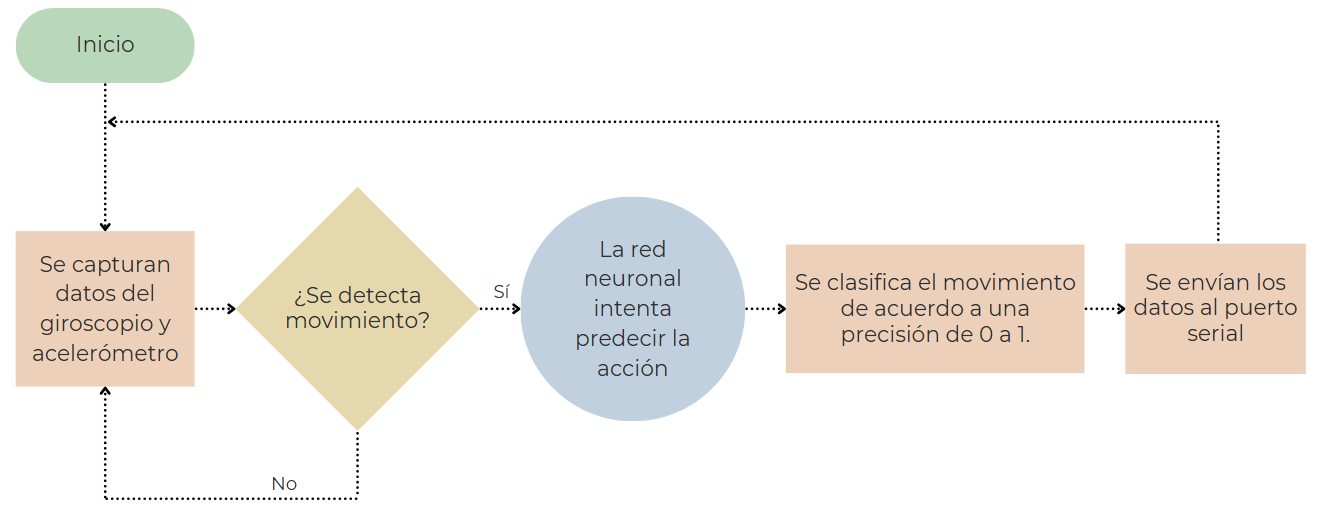
\includegraphics[width=1\linewidth]{Imagenes/diagrama.png}
    \caption{Diagrama de flujo}
    \label{flujo}
\end{figure}

\subsection{Creación del modelo}  
Para la creación del modelo se utilizó la plataforma \textit{Edge Impulse}, lo que requirió la instalación de las herramientas \textbf{arduino-cli} y \textbf{edge-impulse-cli}. Una vez completada la instalación de los programas y paquetes necesarios, se procedió a crear un proyecto en Edge Impulse, nombrado \textit{Laboratorio\_5}.  

El primer paso consistió en conectar el dispositivo Arduino Nano 33 BLE Sense al proyecto. Para lograrlo, se siguieron las instrucciones en la documentación oficial del microcontrolador proporcionada por Edge Impulse \cite{edgeardu}. Tras establecer la conexión correctamente, se pudo comenzar con la recolección de datos. En la Figura~\ref{fig:6} se muestra el Arduino Nano conectado correctamente a la plataforma.  

\begin{figure}[H]
    \centering
    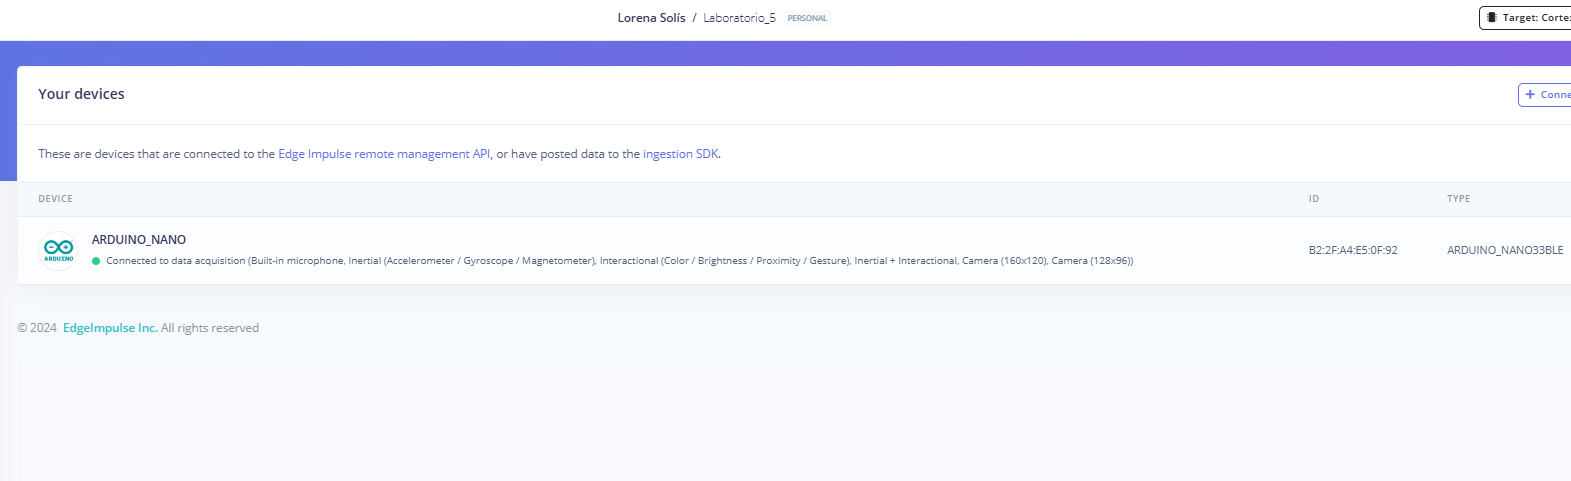
\includegraphics[width=0.8\linewidth]{Imagenes/device.png}
    \caption{Arduino Nano 33 BLE Sense conectado a Edge Impulse.}
    \label{fig:6}
\end{figure}


\subsubsection{Adquisición de datos}
En la sección de \textbf{Data Acquisition} se procedió a grabar los tres movimientos que se desean implementar en el modelo: \textit{arriba-abajo}, \textit{círculo} y \textit{estacionario}. En la Figura~\ref{fig:7}, se observa que el modelo fue entrenado durante un tiempo total de 20 minutos y 37 segundos, incluyendo tanto la fase de pruebas como la de entrenamiento. Además, se utilizó el sensor inercial que utiliza el acelerómetro, giroscopio y magnetómetro del IMU LSM9DS1.

Cada \textit{sample} registrado tuvo una duración de 10 segundos. Se realizaron un total de 40 muestras para los movimientos \textit{círculo} y \textit{arriba-abajo}, mientras que para el movimiento \textit{estacionario} se tomaron 24 muestras, dado que, al ser un movimiento más simple, no requiere tantos datos. Con esta información recopilada, fue posible generar los impulsos necesarios para entrenar el modelo de manera completa.

\begin{figure}[H]
    \centering
    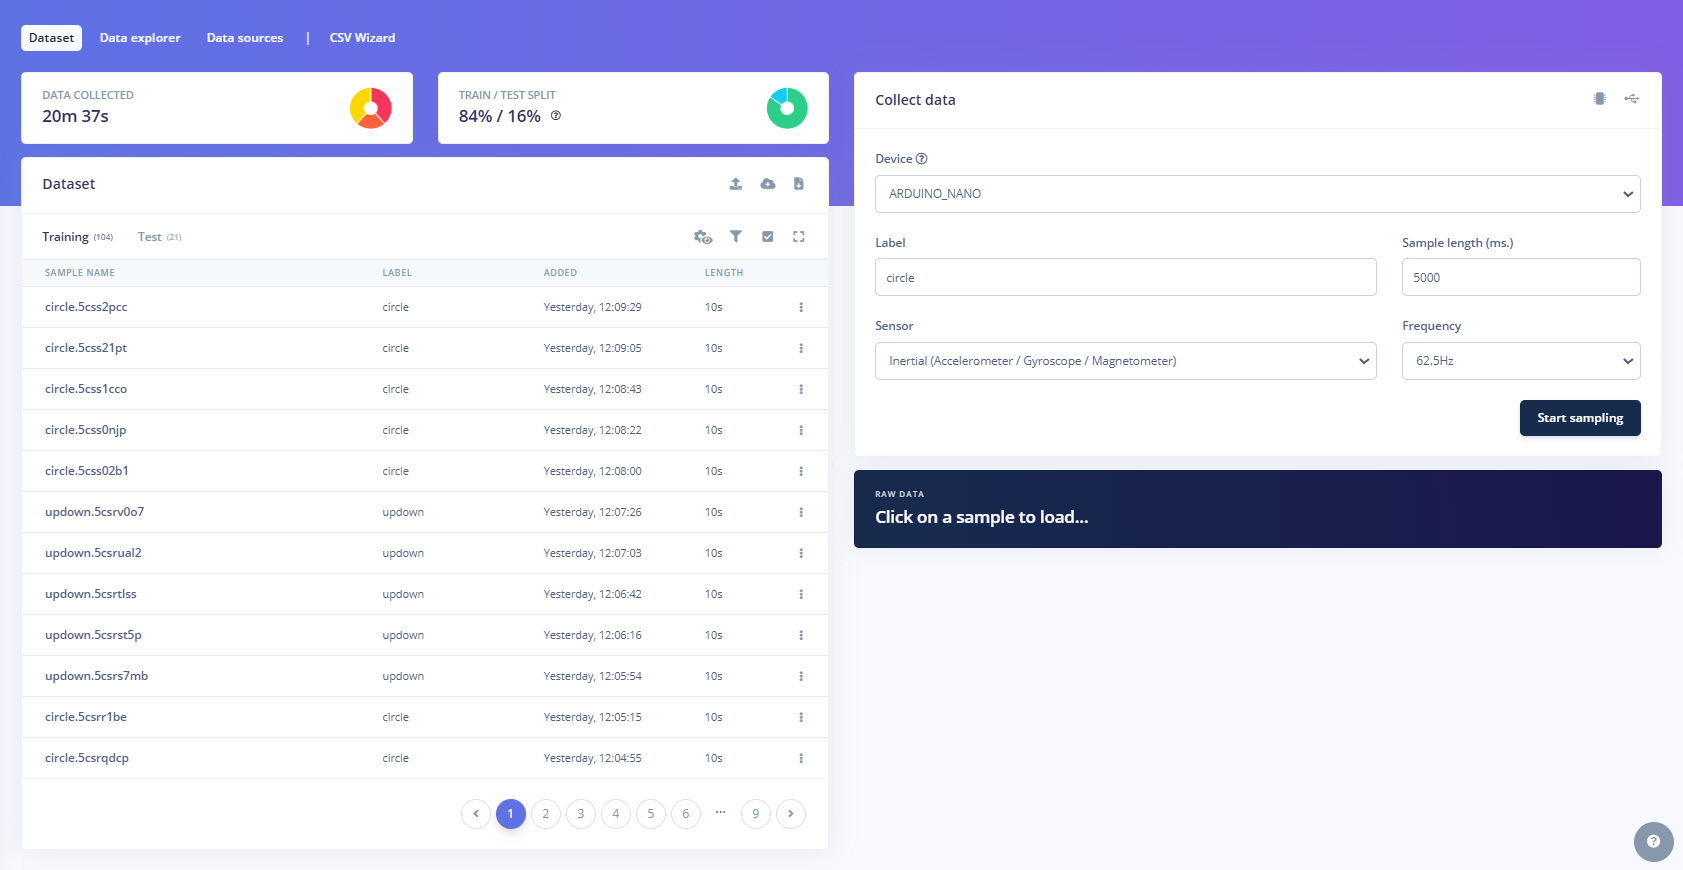
\includegraphics[width=0.8\linewidth]{Imagenes/dataset.png}
    \caption{Set de datos para entrenar y testear el modelo}
    \label{fig:7}
\end{figure}

\subsubsection{Impulsos}

Con el conjunto de datos de entrenamiento listo, se procedió a diseñar un impulso. Un impulso toma los datos crudos, los divide en ventanas más pequeñas, aplica bloques de procesamiento de señales para extraer características, y utiliza un bloque de aprendizaje para clasificar nuevos datos. En el entorno de Edge Impulse, dentro de la sección \textit{Create Impulse}, se configuraron los siguientes parámetros:\\
Tamaño de la ventana: \textbf{2000 ms}.\\
Incremento de ventana: \textbf{80 ms}.\\
Bloques añadidos: \textit{Spectral Analysis}, \textit{Classification} y \textit{Anomaly Detection}.\\
Finalmente, se guardó el diseño del impulso seleccionando la opción \textit{Save impulse}.

\begin{figure}[H]
    \centering
    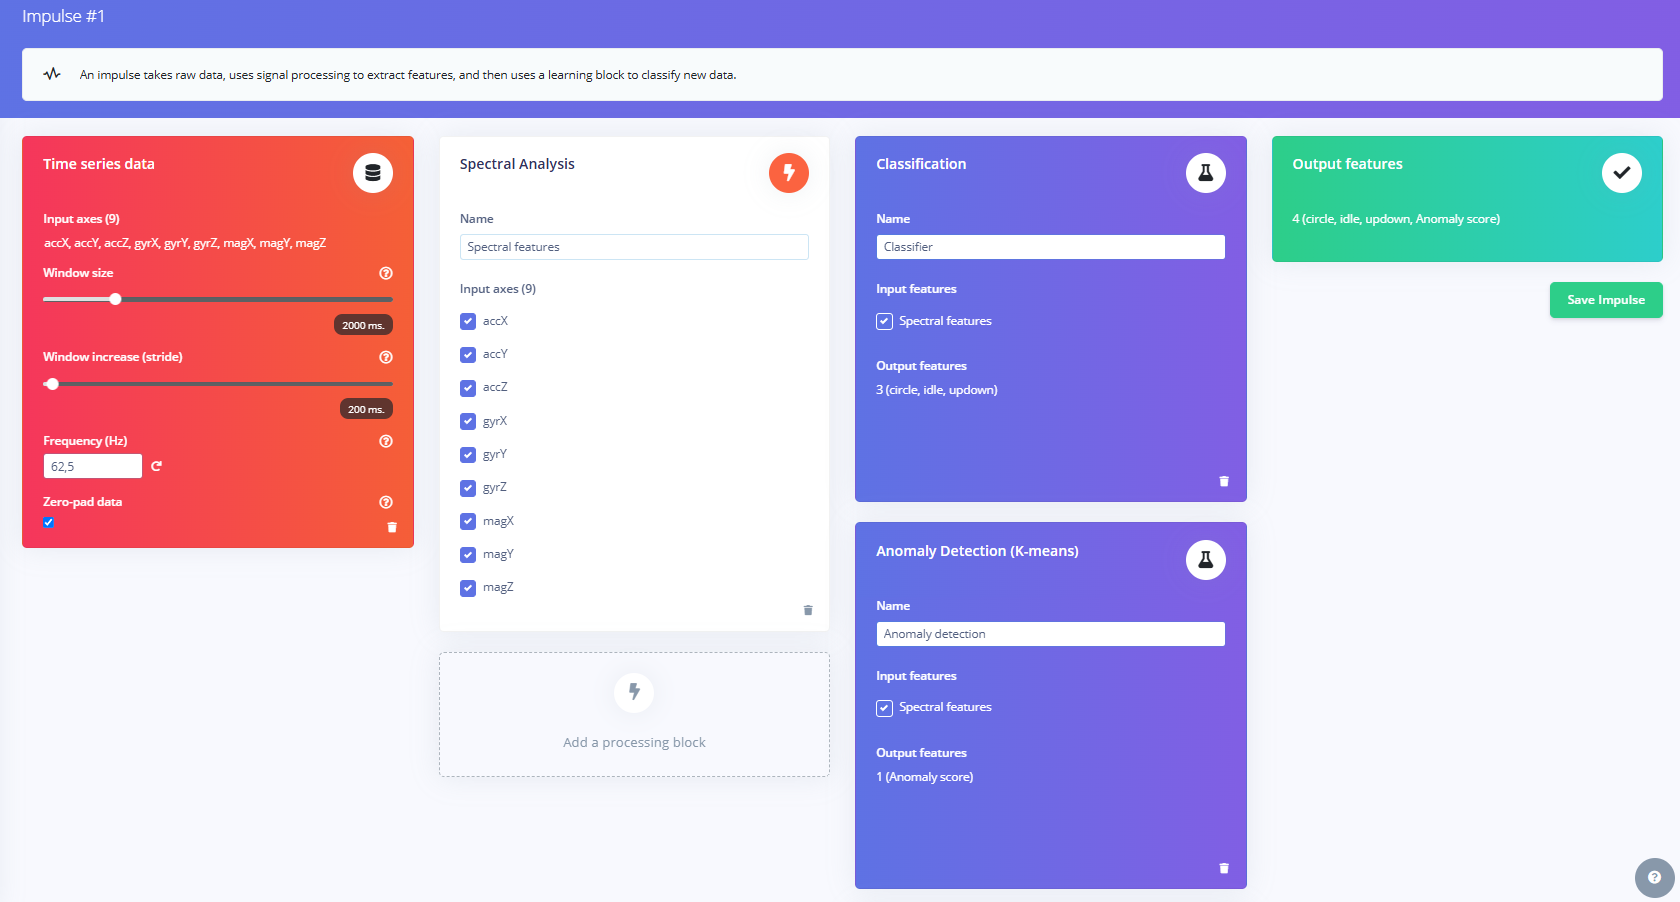
\includegraphics[width=0.7\linewidth]{Imagenes/impulse.png}
    \caption{Impulsos para el entrenamiento del modelo}
    \label{fig:8}
\end{figure}

\begin{itemize}
    \item \textbf{Spectral Features}: El bloque de procesamiento de señales \textit{Spectral Analysis}, el cual aplica un filtro, realiza un análisis espectral sobre la señal y extrae datos relacionados con la frecuencia y la potencia espectral.
    \begin{figure}[H]
    \centering
    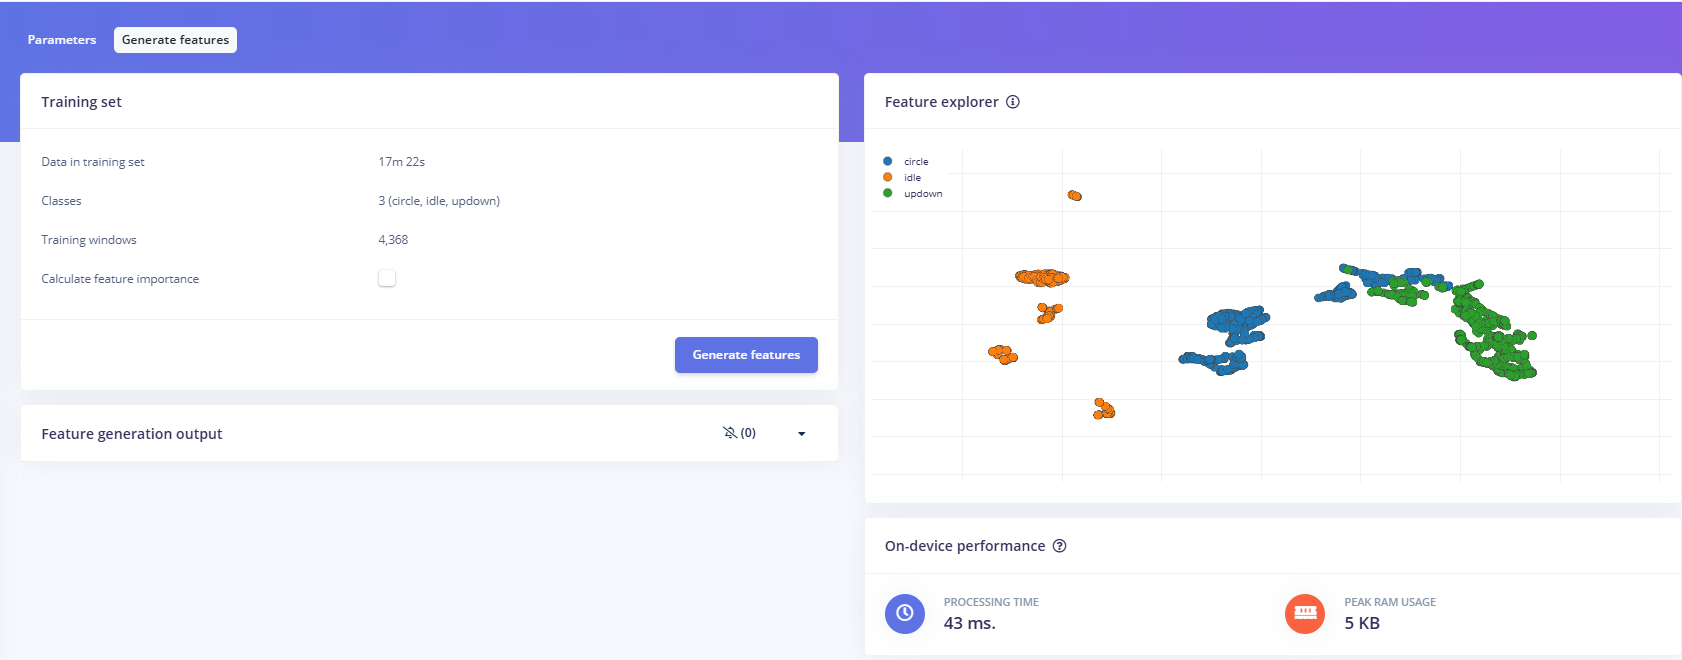
\includegraphics[width=0.8\linewidth]{Imagenes/spectral_features.png}
    \caption{Impulso de características espectrales}
    \label{fig:9}
    \end{figure}
    Como se observa en la figura \ref{fig:9}, al generar las funciones se muestra un gráfico y se observan clusters de cada uno de los movimientos lo que indica que el modelo de ML será capaz de verlo también.

    \item \textbf{Classifier}: El bloque de aprendizaje \textit{Classifier} toma las características espectrales y aprende a distinguir entre las clases definidas (\textit{idle}, \textit{circle}, y \textit{updown}). Para este proceso, se utilizan los siguientes parámetros de configuración:

    \subitem \textbf{Número de ciclos de entrenamiento}: Se configuró para 100 ciclos, lo que implica que el modelo ajusta sus parámetros en 100 iteraciones completas sobre el conjunto de datos de entrenamiento.
    \subitem \textbf{Tasa de aprendizaje}: Se estableció en 0.0005, un valor pequeño que permite una actualización gradual de los pesos de la red neuronal durante el entrenamiento, evitando ajustes demasiado grandes que podrían llevar a un sobreajuste o a una convergencia inestable.
    \subitem \textbf{Tamaño del conjunto de validación}: Se asignó un 60\% de los datos para la validación, lo que permite evaluar el desempeño del modelo en datos no vistos durante el entrenamiento y así detectar posibles problemas de sobreajuste.
    \subitem \textbf{Tamaño del lote (Batch size)}: Se configuró el tamaño del lote en 32, lo que significa que el modelo actualiza sus parámetros después de procesar 32 muestras a la vez.

En la figura \ref{fig:10}, se muestra la clasificación realizada con esta configuración de entrenamiento con un resultado del 99.8\% de exactitud y un 0.02 de perdidas. 

    \begin{figure}[H]
    \centering
    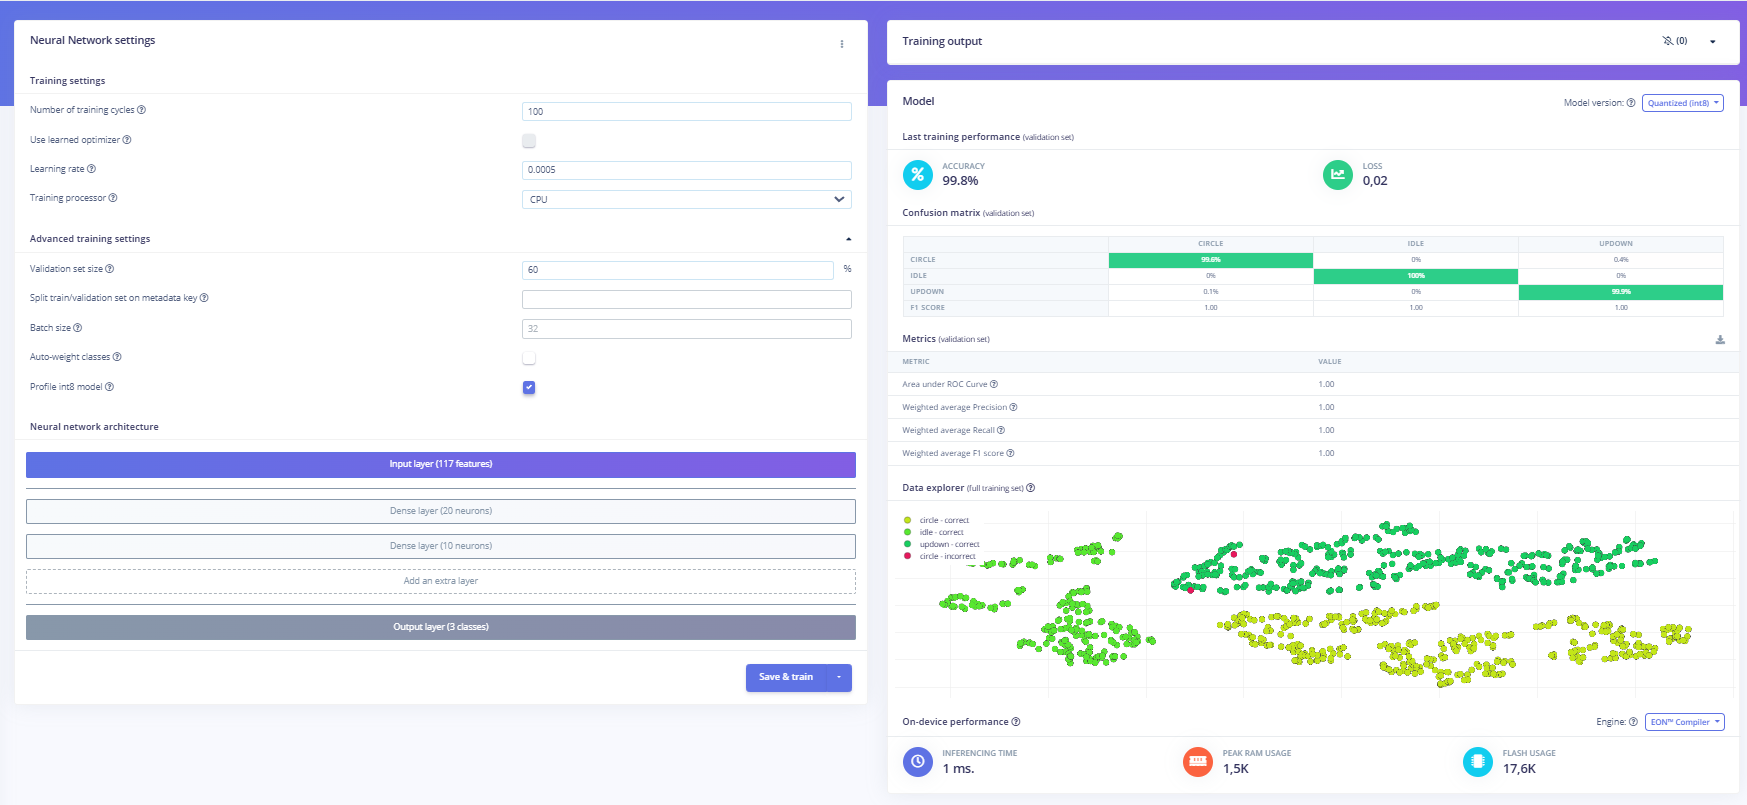
\includegraphics[width=0.8\linewidth]{Imagenes/classifier.png}
    \caption{Impulso de clasificación}
    \label{fig:10}
    \end{figure}


\item \textbf{Anomaly Detection} El \textit{anomaly detection} ayuda a identificar datos que son significativamente diferentes de los que el modelo ha visto durante el entrenamiento. En lugar de clasificar estos datos como uno de los grupos predefinidos, se utiliza un segundo modelo que crea clústeres alrededor de los datos conocidos. Si un nuevo dato se encuentra demasiado alejado de estos clústeres, se considera una anomalía y se marca como no confiable, evitando que el modelo realice una clasificación errónea.
En las imágenes de la Figura~\ref{fig:anomaly_detection} se muestran las anomalías para tres movimientos: En la subfigura \ref{fig:11}, correspondiente al movimiento \textit{updown}, se observan puntos alejados del clúster principal, indicando anomalías.Seguidamente, la subfigura \ref{fig:12}, para el movimiento \textit{idle}, las anomalías se presentan como variaciones fuera del patrón estacionario. Finalmente, en la subfigura \ref{fig:13}, para el movimiento \textit{circle}, se destacan algunas muestras que no siguen el comportamiento esperado de un movimiento circular.
Estas gráficas permiten visualizar cómo el modelo detecta comportamientos anómalos en los diferentes movimientos.

\begin{figure}[H]
    \centering
    % First subfigure
    \begin{subfigure}{0.31\textwidth}
        \centering
        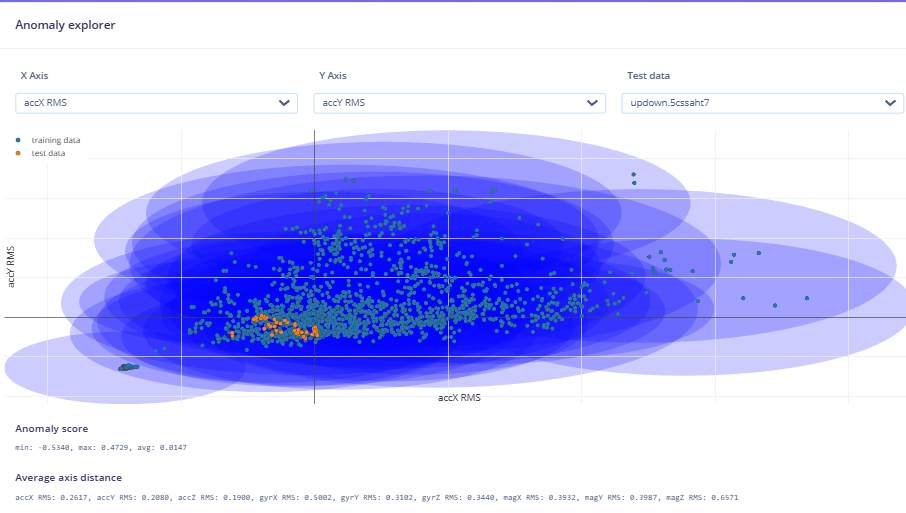
\includegraphics[width=\linewidth]{Imagenes/anomaly_up.png}
        \caption{Anomalías para movimiento updown.}
        \label{fig:11}
    \end{subfigure}
    \hspace{0.02\textwidth} % Add horizontal space
    % Second subfigure
    \begin{subfigure}{0.31\textwidth}
        \centering
        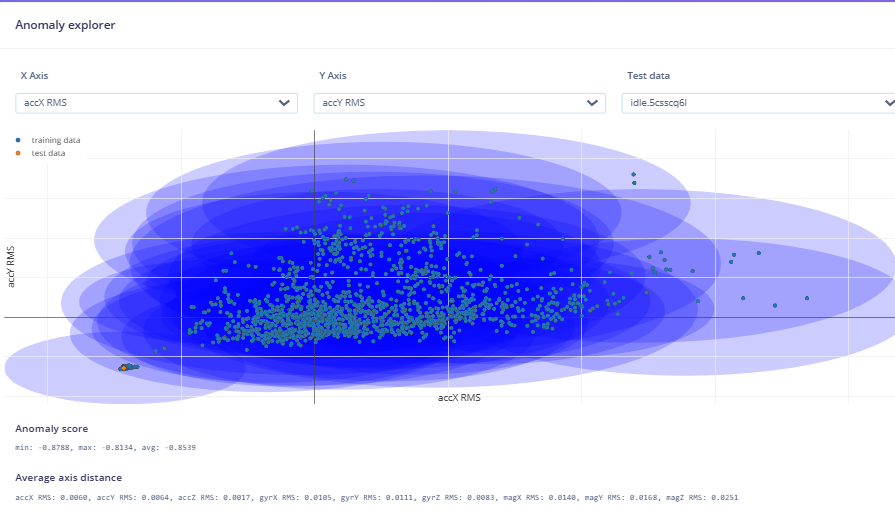
\includegraphics[width=\linewidth]{Imagenes/anomaly_idle.png}
        \caption{Anomalías para movimiento idle.}
        \label{fig:12}
    \end{subfigure}
    \hspace{0.02\textwidth} % Add horizontal space
    % Third subfigure
    \begin{subfigure}{0.31\textwidth}
        \centering
        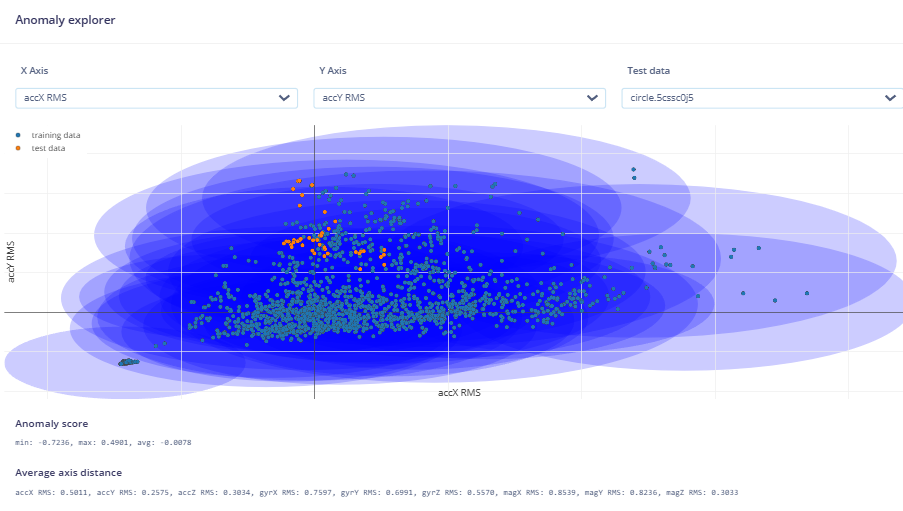
\includegraphics[width=\linewidth]{Imagenes/anomaly_circle.png}
        \caption{Anomalías para movimiento circle.}
        \label{fig:13}
    \end{subfigure}
    \caption{Anomalías detectadas para diferentes movimientos.}
    \label{fig:anomaly_detection}
\end{figure}
    
\end{itemize}

\subsubsection{Clasificación en tiempo real desde Edge Impulse}
En la clasificación en tiempo real, se evaluó cómo el modelo clasifica datos en escenarios nuevos, no vistos durante el entrenamiento. Este análisis permite verificar tanto la precisión como la robustez del modelo frente a datos reales. Para esta evaluación, se tomaron muestras de 10 segundos y 5 segundos, explorando así diferentes modalidades del modelo.

En primer lugar, para el movimiento updown, mostrado en la figura \ref{fig:14}, se observa que el modelo clasifica correctamente la mayoría de las muestras, obteniendo un resultado de 39/42 clasificaciones correctas. Esto corresponde a una exactitud aproximada del $92,8\%$, lo que indica que el modelo no solo identifica adecuadamente el movimiento, sino que también clasifica correctamente las anomalías.

\begin{figure}[H]
    \centering
    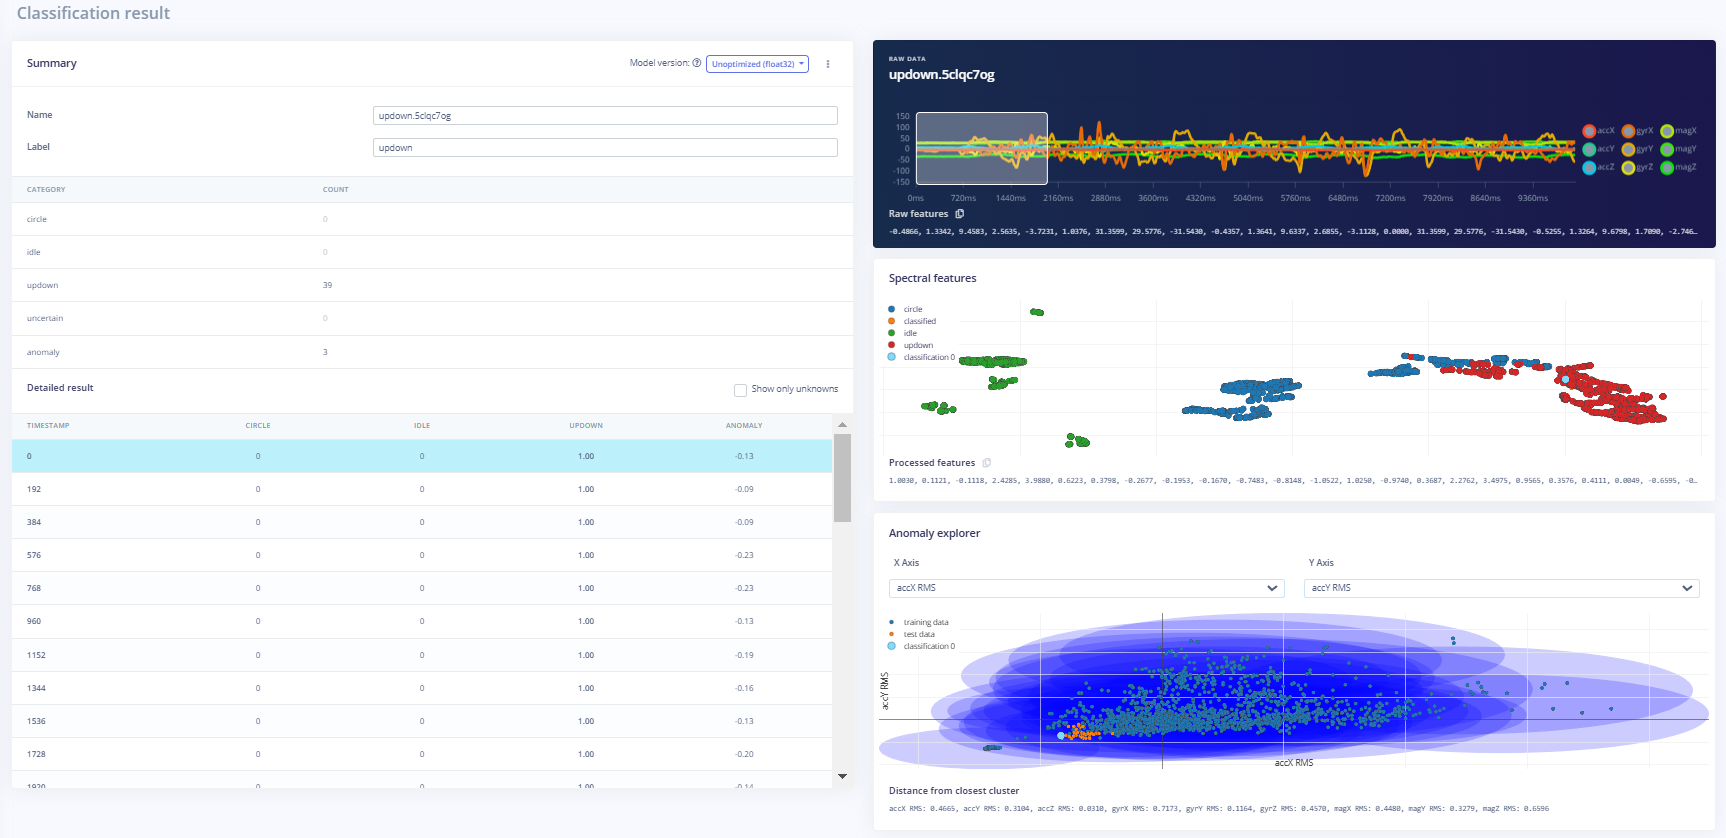
\includegraphics[width=0.6\linewidth]{Imagenes/live_updown.png}
    \caption{Clasificación en tiempo real del movimiento updown}
    \label{fig:14}
\end{figure}

Por otra parte, en la prueba del movimiento idle, representado en la figura \ref{fig:15}, el modelo logró una exactitud del $100\%$, clasificando correctamente las 42 instancias evaluadas. Este resultado demuestra la capacidad del modelo para identificar este tipo de movimiento con total precisión bajo las condiciones de prueba en tiempo real.

\begin{figure}[H]
    \centering
    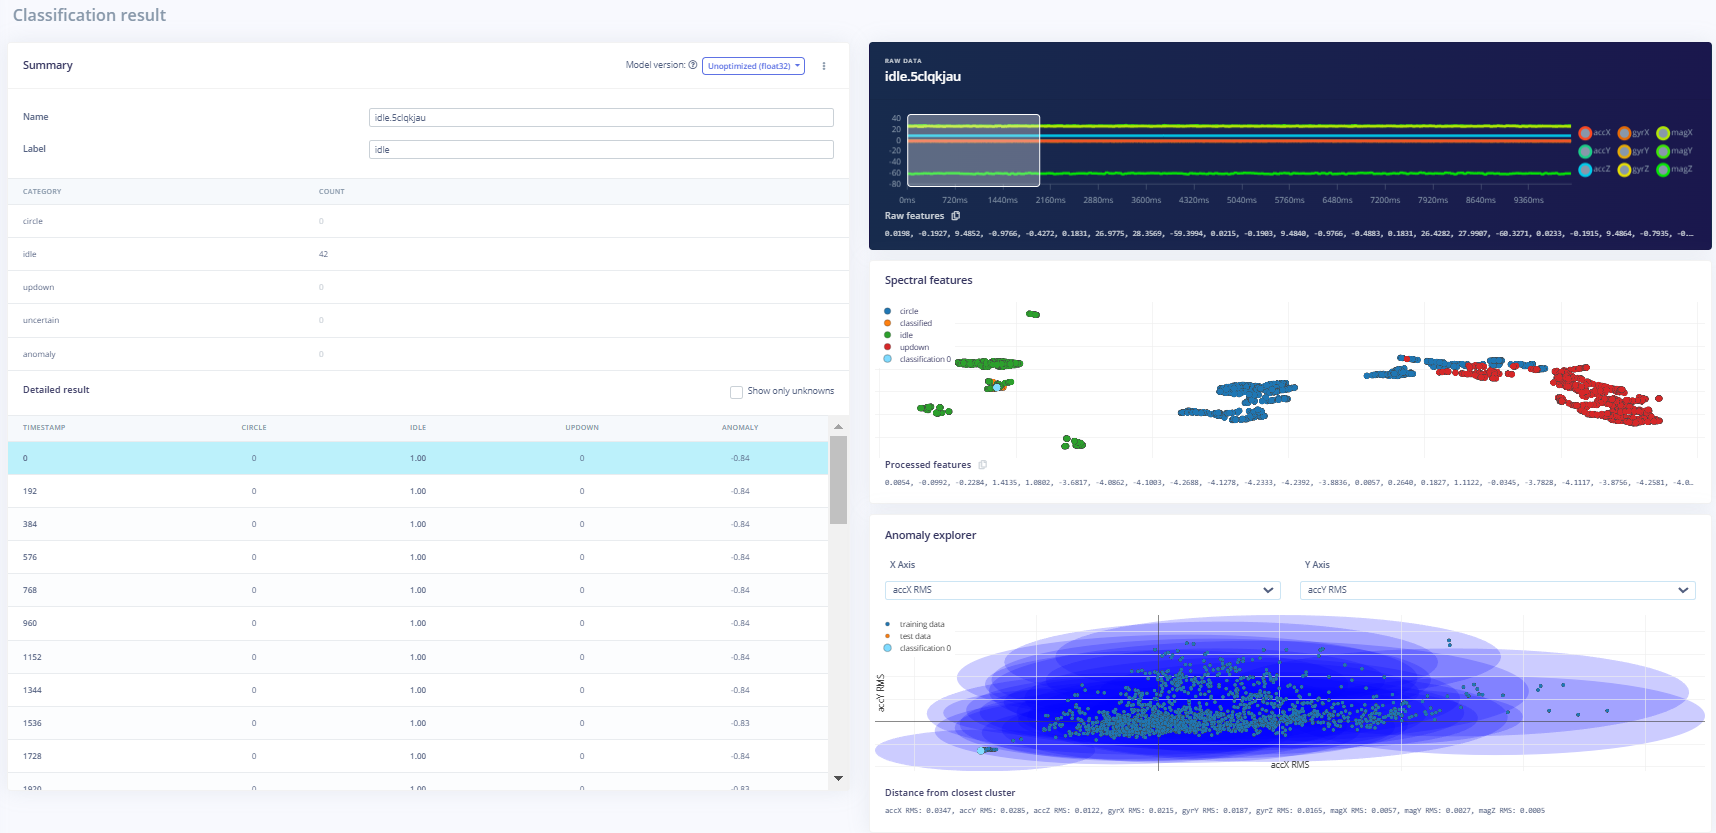
\includegraphics[width=0.6\linewidth]{Imagenes/live_idle.png}
    \caption{Clasificación en tiempo real del movimiento idle}
    \label{fig:15}
\end{figure}

En el caso del movimiento circle, representado en la figura \ref{fig:16}, el modelo alcanzó una exactitud del $97,6\%$, clasificando correctamente 41 de las 42 instancias evaluadas y presentando una única anomalía. Estos resultados reflejan un desempeño sólido en la clasificación en tiempo real de este tipo de movimiento.

\begin{figure}[H]
    \centering
    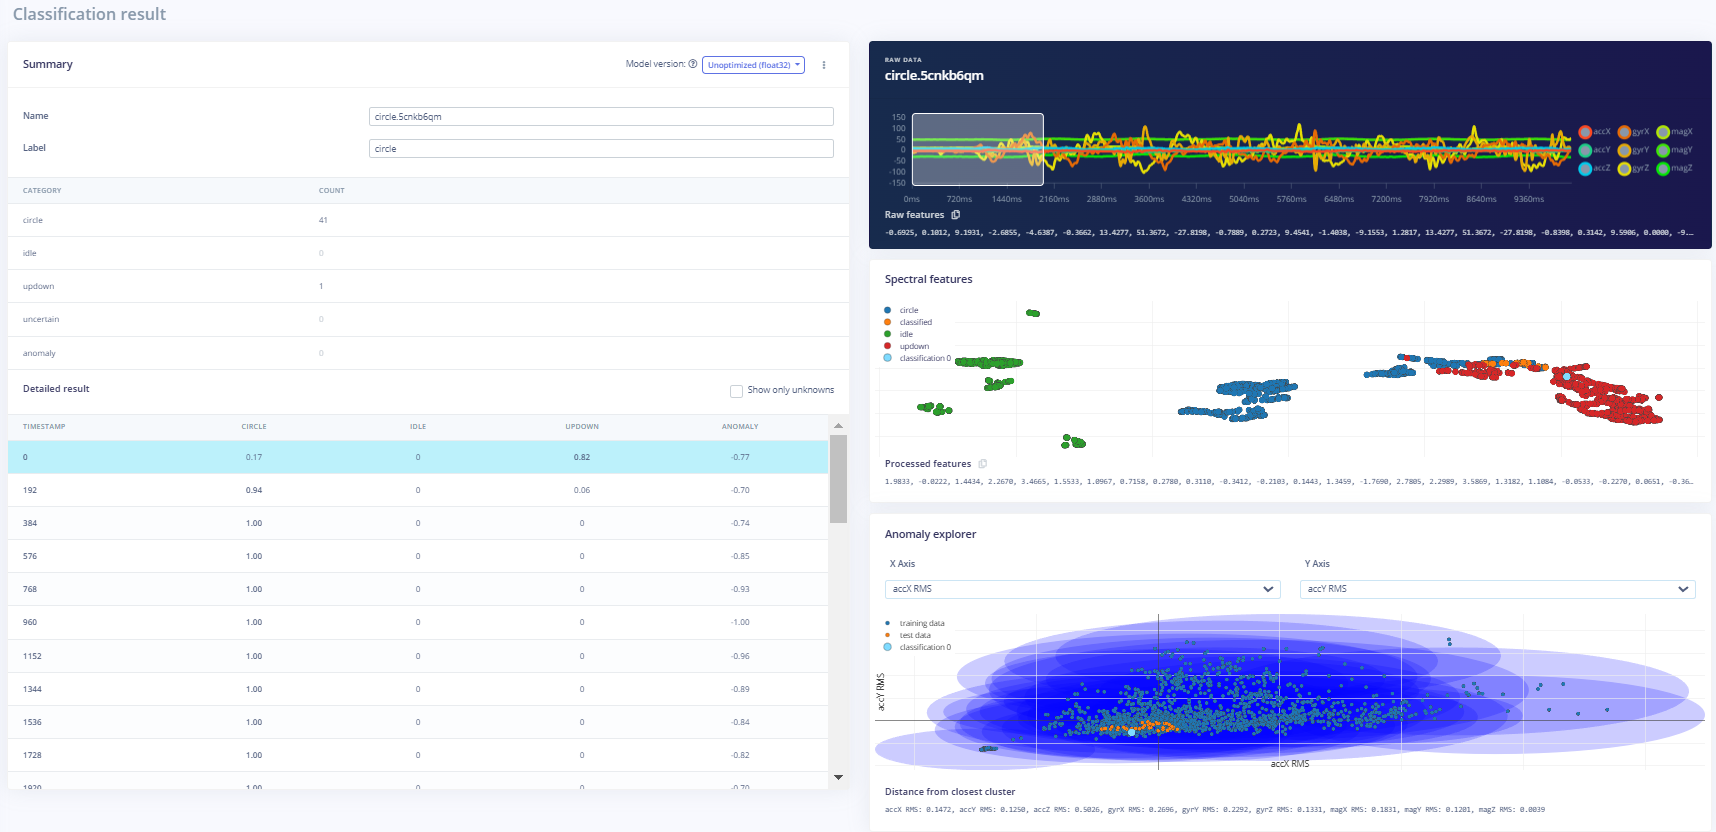
\includegraphics[width=0.6\linewidth]{Imagenes/live_circle.png}
    \caption{Clasificación en tiempo real del movimiento circle}
    \label{fig:16}
\end{figure}

\subsubsection{Prueba de modelo}
Se realizó una prueba final de clasificación antes del deployment, en la cual el modelo evaluó todos los datos obtenidos tanto en la etapa de adquisición de datos (data acquisition) como en la clasificación en tiempo real (live classification) con el propósito de prueba. Esta prueba involucró la ejecución de múltiples clasificaciones de manera simultánea. Como se observa en la figura \ref{fig:17}, el modelo mostró un desempeño exitoso, alcanzando una exactitud del $94,65\%$. Se clasificaron correctamente las anomalías y, en un número reducido de casos, se observaron errores de clasificación.
\begin{figure}[H]
    \centering
    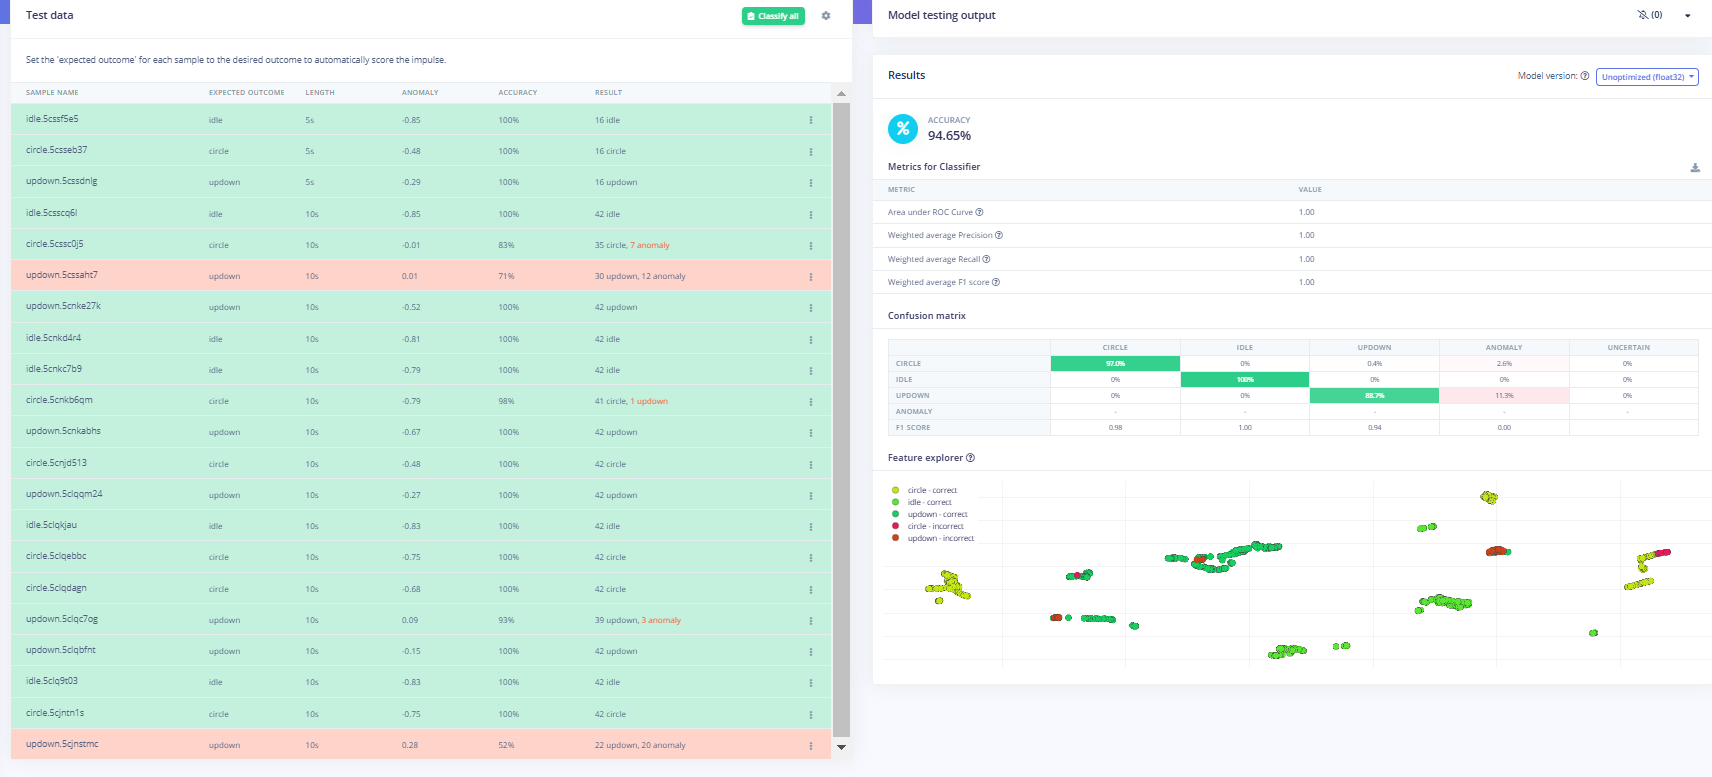
\includegraphics[width=0.8\linewidth]{Imagenes/model_testing.png}
    \caption{Model testing}
    \label{fig:17}
\end{figure}

\subsubsection{Deployment}
Finalmente, se llevó a cabo el deployment en la plataforma Edge Impulse, donde se generó una biblioteca compatible con el entorno de desarrollo Arduino IDE. Esto permitió implementar el modelo en un dispositivo Arduino Nano, logrando obtener resultados de clasificación directamente en el dispositivo sin necesidad de conexión a Internet, garantizando así un funcionamiento autónomo y eficiente.
\begin{figure}[H]
    \centering
    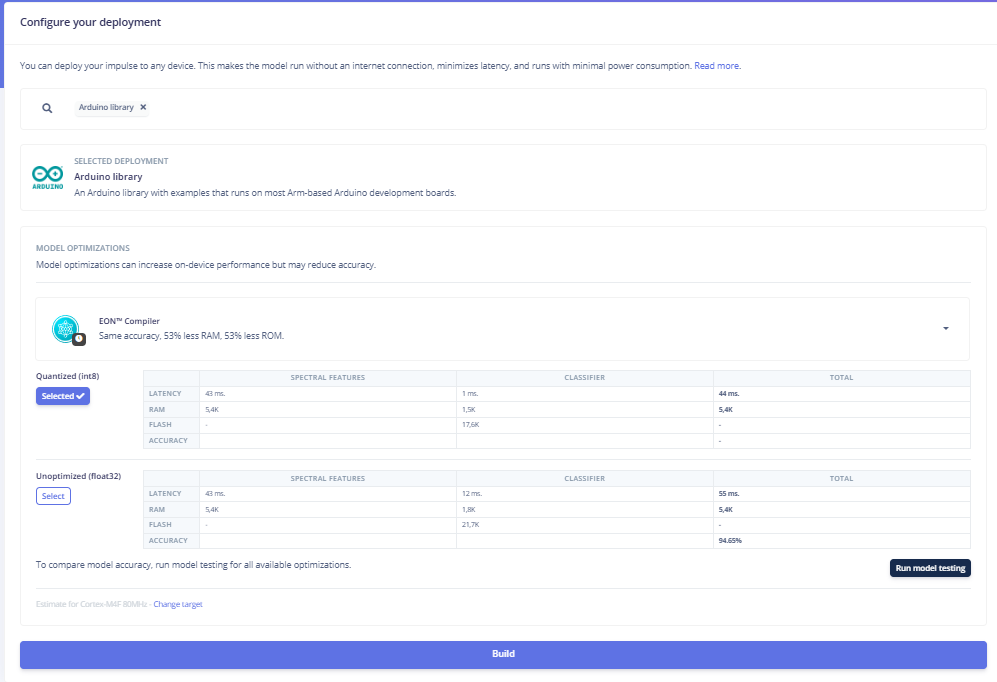
\includegraphics[width=0.6\linewidth]{Imagenes/deployment.png}
    \caption{Creación de la biblioteca para Arduino IDE}
    \label{fig:18}
\end{figure}

\subsection{Resultados}

En la Figura \ref{fig:19} se muestran los resultados obtenidos al ejecutar el modelo de clasificación directamente en el microcontrolador Arduino Nano utilizando la biblioteca generada a partir de Edge Impulse. Durante la inferencia en tiempo real, se realizaron múltiples pruebas para clasificar los movimientos circle, idle y updown, obteniendo las siguientes observaciones:
\begin{itemize}
    \item El modelo clasificó correctamente el movimiento como idle con una confianza del 99.2\%. Aunque se detectó un puntaje de anomalía de -0.622, este valor está dentro de los rangos esperados para el comportamiento normal
    \item En este caso, el modelo clasificó correctamente el movimiento circle con una confianza del 99.6\%. El puntaje de anomalía, de -0.449, confirma que el modelo interpreta adecuadamente este movimiento.
    \item Finalmente, el modelo identificó el movimiento updown con una confianza del 99.6\%. El puntaje de anomalía fue positivo (0.242), pero sigue siendo un valor que valida la robustez del sistema.
\end{itemize}

\begin{figure}[H]
    \centering
    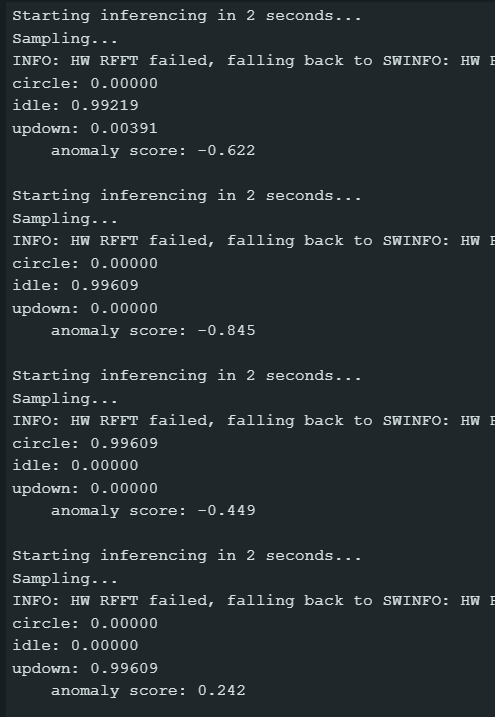
\includegraphics[width=0.5\linewidth]{Imagenes/results_2.png}
    \caption{Resultados con Arduino IDE}
    \label{fig:19}
\end{figure}


\section{Conclusiones y recomendaciones}
\subsection{Conclusiones}  
\begin{itemize}
    \item El modelo alcanzó altos niveles de precisión en la clasificación de los movimientos \textit{circle}, \textit{idle} y \textit{updown}, con exactitudes superiores al 99\% en cada escenario.  
    \item Los puntajes de anomalía obtenidos indicaron un comportamiento consistente, permitiendo identificar con claridad movimientos anómalos o fuera de los patrones esperados.  
    \item La implementación del modelo directamente en el hardware demostró ser eficiente, eliminando la necesidad de conexión a internet para la inferencia y destacando la adaptabilidad del sistema en entornos autónomos.  
\end{itemize}

\subsection{Recomendaciones}  
\begin{itemize}
    \item Preparación del entorno de trabajo: Es fundamental instalar con anticipación todos los programas, controladores y paquetes necesarios para el desarrollo del proyecto, incluyendo Edge Impulse CLI, Arduino IDE, y cualquier otra dependencia requerida. Esto es especialmente importante debido a la complejidad y las posibles incompatibilidades que pueden surgir.  
    \item Gestión de datos en Edge Impulse: Se recomienda planificar cuidadosamente el proceso de adquisición de datos (sampling), ya que ocasionalmente Edge Impulse puede presentar dificultades al registrar muestras, lo que podría afectar la calidad y cantidad de datos recolectados.  
\end{itemize}

\begin{thebibliography}{}
\bibitem{hoja}
Arduino. (2022). \emph{Arduino Nano 33 BLE Sense Product Reference Manual}. SKU: ABX00031.

\bibitem{nRF52840}
Nordic Semiconductor. (2019). \emph{nRF52840 Product Specification}. Version 1.1.  

\bibitem{imu}
STMicroelectronics. (2024). \emph{LSM9DS1 - iNEMO inertial module: 3D accelerometer, 3D gyroscope, 3D magnetometer}.\url{https://www.st.com/en/mems-and-sensors/lsm9ds1.html}

\bibitem{micro}
STMicroelectronics. (2024). \emph{MP34DT05 - MEMS Audio Sensor Omnidirectional Digital Microphone}. \url{https://www.datasheet-pdf.com/datasheet-pdf/view/929317/STMICROELECTRONICS/MP34DT05.html}


\bibitem{cam}
Arduino. (2024). \emph{Arducam Camera Module}. \url{https://store-usa.arduino.cc/products/arducam-camera-module?srsltid=AfmBOoodj96T_OyxRV8OikVgn4KPTsDMR_OBRClfQGnVa8ZW9Zvh_h5P}

\bibitem{sensor}
Avago Technologies. (2024). \emph{APDS-9960 - Digital Proximity, Ambient Light, RGB and Gesture Sensor}.\url{https://www.alldatasheet.com/datasheet-pdf/pdf/918047/AVAGO/APDS-9960.html}

\bibitem{sensor_1}
Nano BLE Sense. (2024). \emph{Nano BLE Sense Digital Proximity, Ambient Light, RGB and Gesture Sensor APDS-9960}. 

\bibitem{edgeardu} 
Edge Impulse (2024), \emph{Arduino Nano 33 BLE Sense - Documentation}.  \url{https://docs.edgeimpulse.com/docs/edge-ai-hardware/mcu/arduino-nano-33-ble-sense}.

\bibitem{ml} 
IBM (s.f.), \emph{¿Qué es machine learning (ML)?}.  \url{https://www.ibm.com/mx-es/topics/machine-learning}.

\bibitem{ei} 
330ohms (2024), \emph{¿Qué es Edge Impulse?}.  \url{https://www.330ohms.com/blogs/blog/que-es-edge-impulse?srsltid=AfmBOorLj5YIWroPbyPYL0d0jBbZskmB3wZKJQkvdZWus_f-05pUvxIC}.

\bibitem{tensorflow} 
incentro (s.f.), \emph{¿Qué es TensorFlow y para qué sirve?}.  \url{https://www.incentro.com/es-ES/blog/que-es-tensorflow}.

\bibitem{lib} 
Arduino Docs (s.f.), \emph{Libraries}.  \url{https://docs.arduino.cc/libraries/}.

\end{thebibliography}



\section{Apéndices}

\includepdf[pages={2-3,5-8,10}]{Documentos/Nano33BLE}
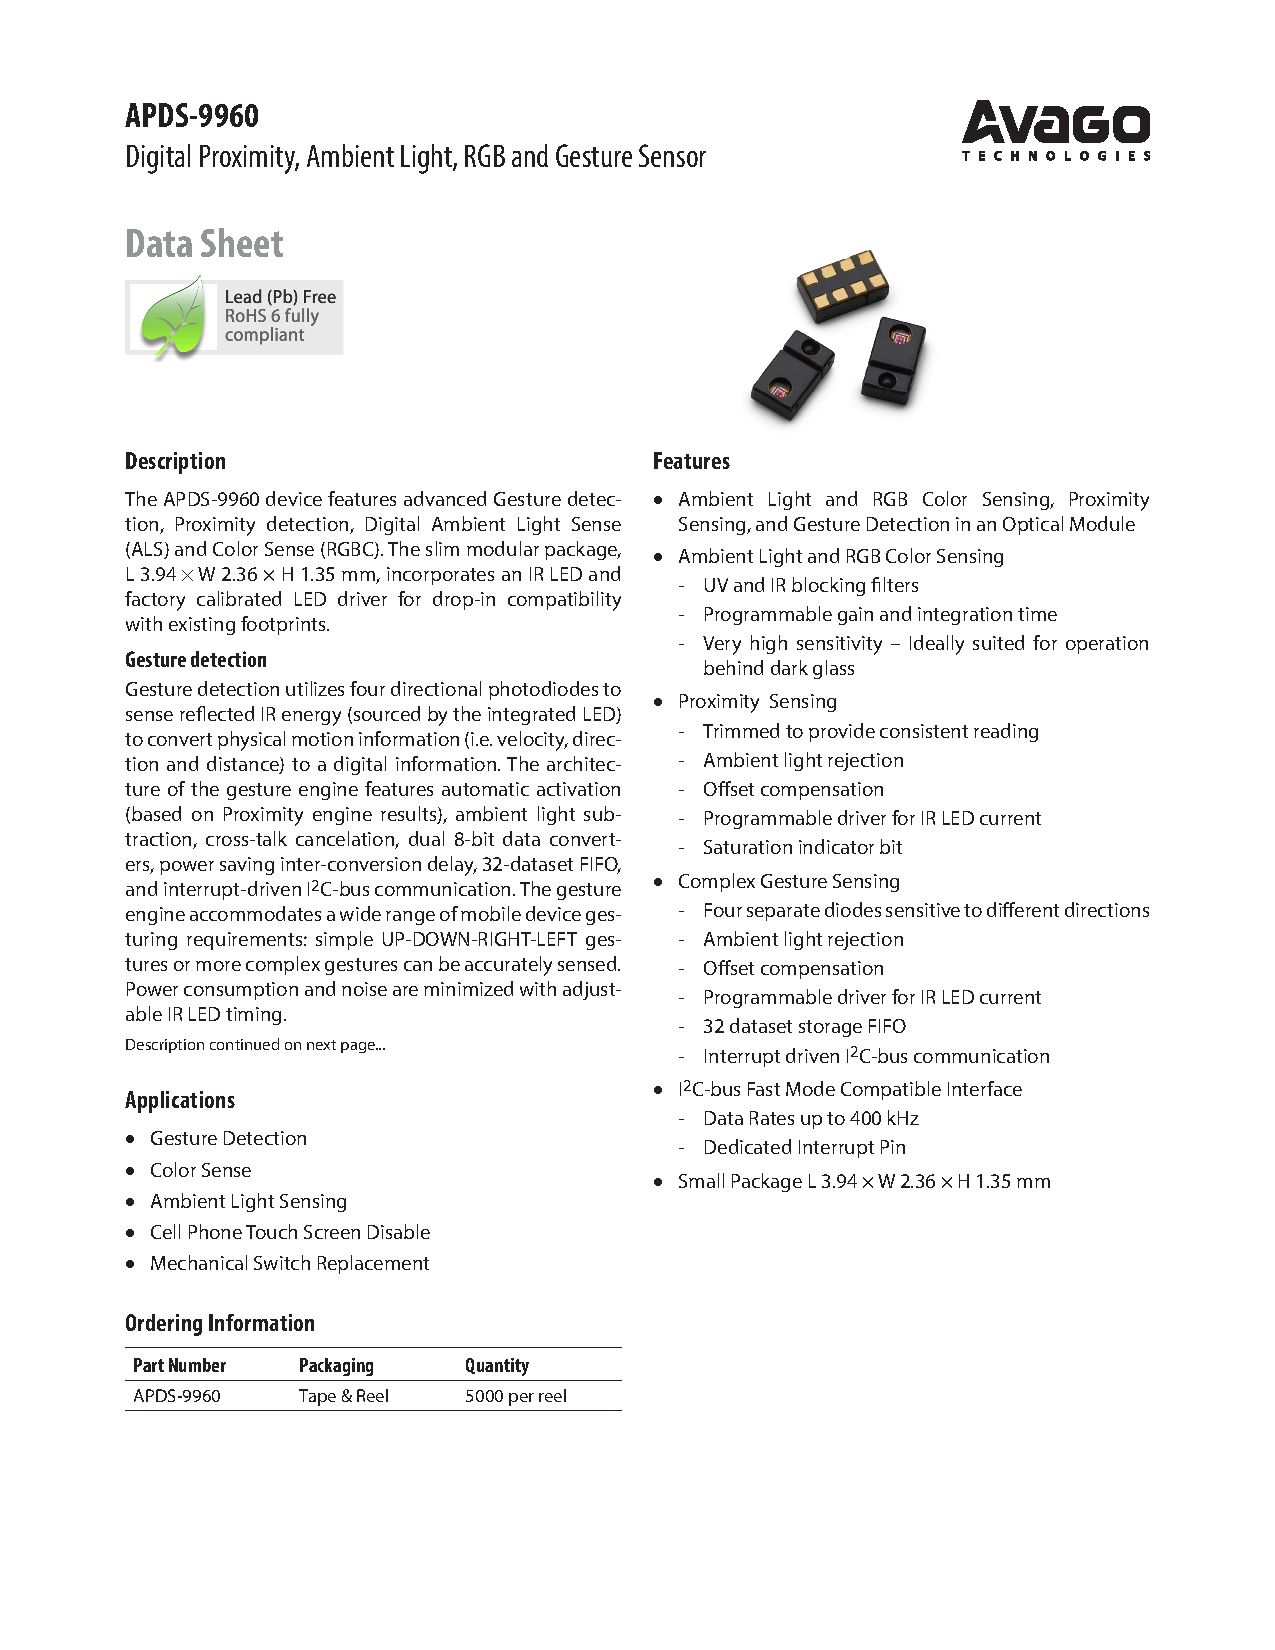
\includepdf[pages={1,2}]{Documentos/Sense_APDS}

\end{document}
